%
% Szakdolgozatminta az Eszterházy Károly Katolikus Egyetem
% matematika illetve informatika szakos hallgatóinak.
%

\documentclass[
% opciók nélkül: egyoldalas nyomtatás, elektronikus verzió
% twoside,     % kétoldalas nyomtatás
% tocnopagenum,% oldalszámozás a tartalomjegyzék után kezdődik
]{thesis-ekf}
\usepackage[T1]{fontenc}
\PassOptionsToPackage{defaults=hu-min}{magyar.ldf}
\usepackage[magyar]{babel}
\usepackage{mathtools,amssymb,amsthm,pdfpages}
\footnotestyle{rule=fourth}

\newtheorem{tetel}{Tétel}[chapter]
\theoremstyle{definition}
\newtheorem{definicio}[tetel]{Definíció}
\theoremstyle{remark}
\newtheorem{megjegyzes}[tetel]{Megjegyzés}

\graphicspath{ {./pictures/} }

\usepackage[normalem]{ulem}
\useunder{\uline}{\ul}{}
\usepackage{float}
\usepackage{pifont}

\usepackage{listingsutf8,xcolor,caption}
\lstset{
	inputencoding=utf8/latin2,
	language=delphi,
	basicstyle=\footnotesize,
	numbers=left,
	breaklines,
	postbreak=\hbox{$\color{red}\hookrightarrow\ $},
	xleftmargin=1cm,
	xrightmargin=1cm,
	backgroundcolor=\color{gray!15},
	frame=tlbr,
	framesep=3pt,
	keywordstyle=\bfseries\color{blue},
	commentstyle=\itshape\color{teal}
}
\renewcommand{\lstlistingname}{kód}


\begin{document}
\institute{Matematikai és Informatikai Intézet}
\title{Adatbázis alapú web alkalmazás fejlesztése}
\author{Lázár Benedek\\Programtervező informatikus BSc}
\supervisor{Dr. Tajti Tibor Gábor\\egyetemi docens}
\city{Eger}
\date{2023}
\maketitle
\tableofcontents

\chapter*{Bevezetés}
\addcontentsline{toc}{chapter}{Bevezetés}

A szakdolgozatom témája egy adatbázisra épülő webes alkalmazás fejlesztése. Gyakran használunk ilyen alkalmazásokat, gondoljunk például a YouTube-ra, vagy a Facebook-ra, ami rengeteg felhasználónak ad lehetőséget, hogy videóit és gondolatait megossza másokkal. Ezeket az adatokat egy adatbázisban tárolják, így a felhasználók feltölthetik ide fájljaikat, vagy letölthetik a mások által feltöltött tartalmakat.

A projektem célja, létrehozni egy adatbázisra épülő webalkalmazást, amelyben a felhasználók csoportokat hozhatnak létre, vagy csatlakozhatnak már meglévő csoportokhoz és ezen belül tudják megosztani egymás között a képeiket és gondolataikat.

A projekt implementálása előtt meg kellett terveznem az alkalmazást és kiválasztani azokat a technológiákat, amiket használni fogok a fejlesztés során.

\vspace{5mm}

Először is szükségem volt egy fejlesztői környezetre, én a Visual Studio Code-ot választottam. Szükségem volt még webszerverre és egy adatbázisra is, és mivel a XAMPP és a PhpMyAdmin könnyen használható, és legtöbbször ezeket használtuk a gyakorlatok során, ezért rájuk esett a választás.

A fejlesztés segítése és gyorsítása érdekében érdemes keretrendszert is használni, én pedig a Laravel keretrendszert használtam, mert ezt a technológiát már ismertem és gyorsan illetve átláthatóan lehet vele dolgozni, ezen kívül rengeteg beépített funkció segítette a munkámat.

Ezeken kívül a verziókövetéshez SourceTree-t, a feladatok kiosztásához és nyomon követéséhez pedig Trello-t használtam.
Annak érdekében, hogy akár XAMPP használata nélkül is lehessen futtatni az alkalmazást és az adatbázist, létrehoztam konténereket is Docker desktop segítségével.

\vspace{5mm}

Az alkalmazás a következő GitHub repository linkről tölthető le:


\url{ https://github.com/benedeklazar/Szakdolgozat_HDMIJ3_2023
}

\chapter{Adatbázis alapú web alkalmazások}
\section{Bevezetés}

Ebben a fejezetben fogom bemutatni az adatbázisok és webalkalmazások általános tulajdonságait, illetve bemutatok néhány olyan web alkalmazást is, amely adatbázisban tárolja az adatait. 

\section{Az internet fejlődése}

Az internet megjelenésével és fejlődésével az emberek gyorsabban és hatékonyabban képesek kapcsolatba lépni más emberekkel, tartalmakat oszthatnak meg egymással és sokan már a munkájukat is internet segítségével végzik. Az Email megjelenésével az embereknek már nincs szükségük valódi levelekre, mert ezek szállítása sokkal több időt és erőforrást vesz igénybe, mint egy elektronikus levél elküldése az interneten keresztül. A közösségi weboldalaknak köszönhetően az emberek felvehetik a kapcsolatot távol levő ismerőseikkel, vagy akár idegenekkel is egy pillanat alatt. Az internetről vásárolhatunk könyveket, ruhákat, vagy akár rendelhetünk ételeket is, anélkül, hogy el kéne hagynunk a otthonunkat. Megtekinthetjük a legújabb híreket, videókat és eseményeket, de használhatjuk tanulásra, vagy játékra is.

Az internet nagyon hasznos, de sajnos megvannak a maga veszélyei is. Ilyenek lehetnek például az internetes átverések, vagy csalások. Az internet növekedésével párhuzamosan a hacker-ek elkezdtek olyan vírusokat írni, amelyek interneten keresztül is terjednek. Fontos, hogy ezeket a csalásokat észrevegyük és ne töltsünk le gyanús weboldalakról fájlokat, vagy szoftvereket, illetve ne vásároljunk termékeket megbízhatatlan oldalakról. De az internetnek más veszélyei is lehetnek a társadalomra, mivel az embereknek az internet kora óta egyre kevesebb mozgásra van szükségük, hiszen bármit elérhetnek otthonról egy kattintással, ha tudnak csatlakozni az internethez. Sokan már iskolába sem járnak, hiszen online is tudnak csatlakozni az oktatáshoz.

\begin{figure}[H]
	\centering
	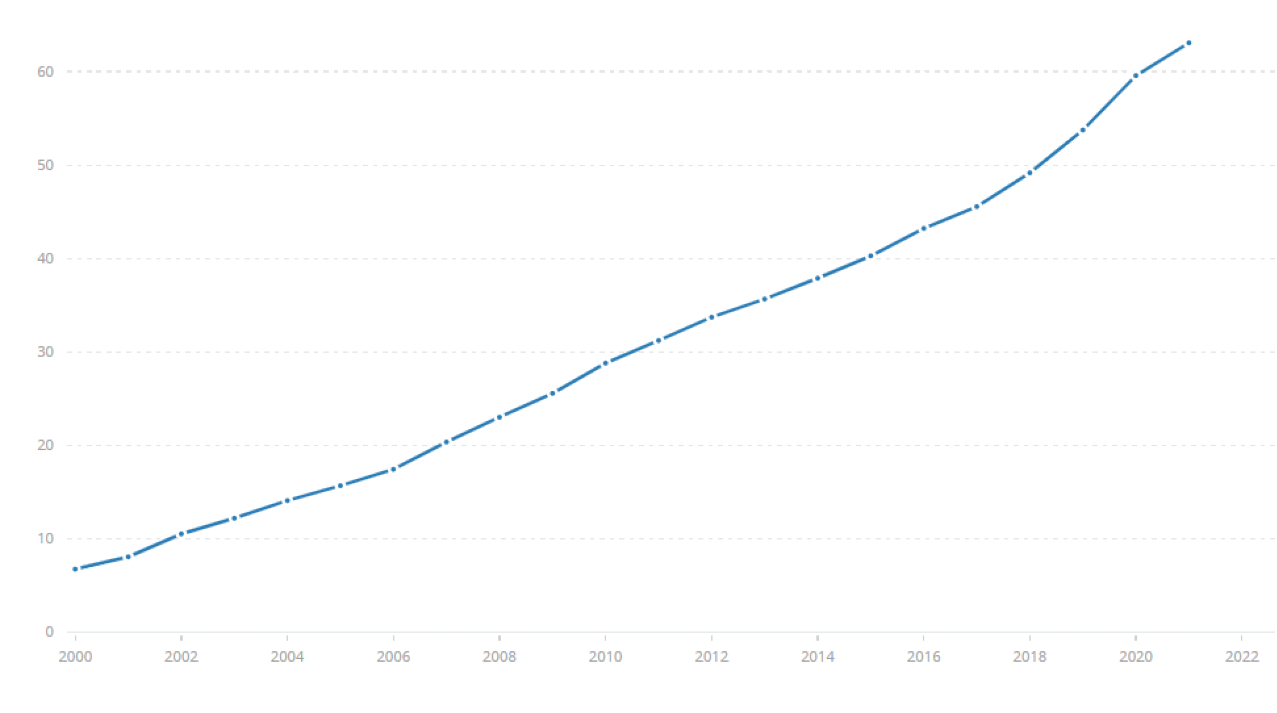
\includegraphics[width=12cm, height=8cm]{internet}
	\caption{Az internetet használó személyek százalékos aránya a világon}
	\label{fig:picture}
\end{figure}

Összességében elmondható, hogy az internetnek köszönhetően rengeteg új munkalehetőség jött létre, gondoljuk a Webfejlesztőkre, vagy akár a YouTube tartalomgyártókra. A weboldalak utat nyitottak a hirdetőknek is, hogy termékeiket mások weboldalain hirdessék, ezáltal a weboldal tulajdonosa bevételhez juthat.

\section{Web alkalmazások}

A webalkalmazások olyan szoftverek, amelyek a böngészőnkben futnak. A web alkalmazásokat bárki használni tudja, akinek van számítógépe és képes csatlakozni az internetre. Ezeket az alkalmazásokat nem kell a számítógépünkre külön telepíteni, hanem gyakran egy távoli szerveren futnak. A legtöbb nem webes szoftverrel az a probléma, hogy telepíteni kell, amely sok tárhelyet és erőforrást vesz el a számítógépünktől. Ezen kívül minden frissítésnél le kell tölteni és telepíteni kell a szoftver egy újabb verzióját. Pozitívum, hogy az ilyen alkalmazásoknak általában nincs szükség internetkapcsolatra a használatukhoz és a felhasználói élmény is gazdagabb. Ezeket a nem webes alkalmazásokat \textbf{vastag kliensnek} is nevezik, szemben a webes alkalmazások kliensével, melyet \textbf{vékony kliensnek} neveznek. A vékony klienshez szükség van egy weboldalra és egy böngészőre, amiben az alkalmazást futtatjuk.
Főbb előnyei a nem webes szoftverekkel szemben a kis hardverigény és az automatikus frissítés.

\section{Adatbázisok}

Az adatbázisok elektronikusan elérhető, logikailag összetartozó információk és adatok szervezett gyűjteménye. Egy adatbázis táblákból, a táblák pedig mezőkből épülnek fel. Minden táblában szükség van egy elsődleges kulcsra, ez az azonosító. Minden egyes rekordnak egy egyedi azonosítót kell biztosítani, azaz nem szerepelhet egy azonosítóból több egy táblában. Ez azért fontos, hogy az adatokra egyértelműen lehessen hivatkozni. Léteznek relációs és nem relációs adatbázis kezelő rendszerek. A legnépszerűbb relációs adatbázis kezelő rendszerek közé tartozik a MySQL, amely SQL nyelvet használ az adatok lekérdezésére.
\\\\
Az adatbázisoknak biztosítani kell az adatok elérhetőségét és védelmét. Oda kell figyelnünk, hogy az érzékeny adatokat, például jelszavakat megfelelő biztonsággal tároljuk, ezért a jelszavakat csak hash-elés után mentjük le az adatbázisban. 
\\\\
Az adatok tárolása, titkosítása és védelme mellett biztosítanunk kell, hogy az adminisztrátorok könnyen hozzáférhessenek az adatokhoz. Lehetőséget kell adni, hogy az adatok bármikor létrehozhatóak, megtekinthetőek, törölhetőek és szerkeszthetőek legyenek az adminisztrátorok számára.

\section{Közösségi média platformok}

Mivel a projektem is egy adatbázisra épülő közösségi média alkalmazás, ezért itt bemutatom ezen alkalmazások főbb tulajdonságait. A közösségi média alkalmazások az emberek interakcióin alapszanak. Létezhetnek híroldalak, melyek napról napra információval szolgálnak. A felhasználók hozzászólás formájában fejezhetik ki véleményüket. A blog oldalakon a felhasználók saját cikkeket és bejegyzéseket hozhatnak létre. Ezek lehetnek oktató jellegűek, humorosak, de akár kritikusak is. A közösségi oldalakon a felhasználók megoszthatják másokkal videóikat, vagy fotóikat.
\\\\
Ezeknek az oldalaknak általában megvannak a saját közösségi irányelveik, melyeket minden felhasználónak be kell tartania. Nem oszthatunk meg akármit, csak olyan tartalmakat, melyek megfelelnek a platform szabályainak. Fontos, hogy ne osszunk meg személyes adatokat, például a jelszavunkat, mert ezeket az információkat bárki láthatja.

\section{Hasonló alkalmazások}
\subsection{Facebook}

A Facebook az egyik legnépszerűbb közösségi hálózat, fő alapítója Mark Zuckerberg. Az alkalmazás felhasználói regisztráció, vagy bejelentkezés után kapcsolatba léphetnek a többi felhasználóval, létrehozhatnak eseményeket, csoportokat és üzleteket. Ismerősnek jelölhetnek más felhasználókat, vagy elfogadhatják a beérkező ismerősnek jelöléseket. A felhasználók megoszthatnak képeket és videókat ismerőseikkel, vagy reagálhatnak mások posztjaira megjegyzés és "tetszik" formájában.

\subsection{YouTube}

A YouTube a legismertebb videómegosztó platform, három alapítója Steve Chen, Chad Hurley és Jawed Karim. Havonta több mint 1 milliárd aktív felhasználója van. Az első videó 2005 április 24.-én került fel a platformra "Me at the zoo" címmel. A YouTube sokak számára munka és pénzkeresési lehetőséget biztosít, mivel a felhasználók akár bevételt is kereshetnek videók feltöltésével, a videókon megjelenő reklámokon keresztül. A platform főbb funkciói közé tartozik a videó feltöltése, lájkolás (tetszik), diszlájkolás (nem tetszik), hozzászólás írása, de létrehozhatunk lejátszási listákat is. A videóknak megadhatunk címet, indexképet és leírást is, illetve bármikor szerkeszthetjük, vagy törölhetjük a videóinkat.

\subsection{Twitter (X)}

A Twitter, vagy "X" egy ismert közösségi hálózat és mikroblog szolgáltatás, négy alapítója Jack Dorsey, Noah Glass, Biz Stone és Evan Williams, jelenlegi tulajdonosa pedig Elon Musk. Az "X", régebben twitter felhasználói rövid szöveges posztokat hozhatnak létre, vagy mások bejegyzéseit oszthatják meg. Népszerű platform a hírességek és cégek körében, hiszen könnyen felvehetik a kapcsolatot követőikkel, felhasználóikkal. Havonta 328 millió felhasználó használja aktívan a platform különböző szolgáltatásait. Főbb szolgáltatásai közé tartozik a "Tweetelés", vagyis egy új poszt létrehozása, a "Re-tweetelés", vagyis egy meglévő poszt újra posztolása, de ezeken kívül van lehetőség hozzászólást írni és lájkolni is. A felhasználók a szöveges posztokhoz mellékelhetnek képeket, vagy videókat is.

\section{Összegzés}

A fent említett adatbázis alapú web alkalmazások inspirálták a szakdolgozatomhoz készült projektet is. A legtöbb ilyen alkalmazás adatbázist használ az adatok tárolására. A projektemben (a Facebook-hoz hasonlóan) létre lehet hozni csoportokat és ezeken belül posztokat megosztani. A posztokra hozzászólás formájában tudnak a felhasználók reagálni. A YouTube fellebbezés rendszeréhez hasonlóan, a felhasználók képesek vitatni valamely tartalmuk eltávolítását, ha azt nem érzik jogosnak. A designt főleg a Twitter és a Facebook inspirálta, ahol a posztok egymás után jelennek meg egyesével.

\chapter{Fejlesztői dokumentáció}
\section{Követelmény specifikáció}
\subsection{Bevezetés}

Ebben a fejezetben fogom összefoglalni az alkalmazásom főbb céljait és követelményeit. Bemutatom a jelenlegi helyzetet, a vágyálom rendszert és az üzleti folyamatok modelljét.

\subsection{Az alkalmazás célja}

Az alkalmazás célja, hogy a felhasználók különböző csoportokat hozzanak létre, vagy meglévő csoportokhoz csatlakozzanak, posztokat és hozzászólásokat hozzanak létre és ezáltal megosszák egymás között gondolataikat. Fontos, hogy a megosztott tartalmakhoz csak azok a felhasználók férjenek hozzá, akiknek megvan hozzá a megfelelő jogosultsága. A felhasználóknak legyen lehetőségük létrehozni, megtekinteni, szerkeszteni és törölni posztjaikat és csoportjaikat. 

\subsection{Jelenlegi helyzet}

Napjainkban a legtöbb közösségi média felület ugyanazokat a tartalmakat fogja ajánlani minden felhasználónak, ezért a tematikus tartalmak gyakran csak kevés emberhez jutnak el. Az algoritmus azokat a tartalmakat fogja népszerűsíteni, amik a többség számára érdekesek lehetnek, emiatt a kevésbé népszerű témák háttérbe szorulnak, és nehezebben találják meg azok, akiket tényleg érdekel az adott téma.

Célunk, hogy az érdeklődők csatlakozhassanak egy kis közösségbe, ahol láthatják, hogy mások milyen tartalmakat osztottak meg a csoportban, miközben ne zavarjuk azokat, akiket nem érdekel az adott téma. Ez azt jelenti, hogy egy csoportban megosztott poszt csak ott lesz elérhető, és csak a tagok tekinthetik meg.

\subsection{Vágyálomrendszer}

Projektünkben a funkciók eltérőek attól függően, hogy mely csoportoknak vagyunk tagjai, például egy tag kevesebb funkciót érhet el, mint egy moderátor, de többet, mint egy olyan felhasználó, aki nem tagja a csoportnak, vagy nincs bejelentkezve.

Szükség van egy magasabb szintű felhasználóra, azaz egy adminisztrátorra, aki korlátlanul hozzáfér minden csoporthoz, poszthoz és felhasználóhoz, azokat szabadon szerkesztheti vagy törölheti.
\\\\
Ha bejelentkezek és létrehozok egy csoportot, akkor azon a csoporton belül én leszek az Admin, azaz kezelhetem, hogy kik csatlakozhatnak a csoportomba, illetve moderálhatom a csoportban megjelenő posztokat. Kijelölhetem a csoport moderátorait, akik segítenek a szabályaim betartatásában.

\subsection{Üzleti folyamatok modellje}

Ha nem vagyunk bejelentkezve, akkor csak a regisztrációra és bejelentkezésre van lehetőségünk. Ha a felhasználó megpróbál valamilyen egyéb műveletet végrehajtani, vissza lesz irányítva a kezdőoldalra.

\begin{figure}[H]
	\centering
	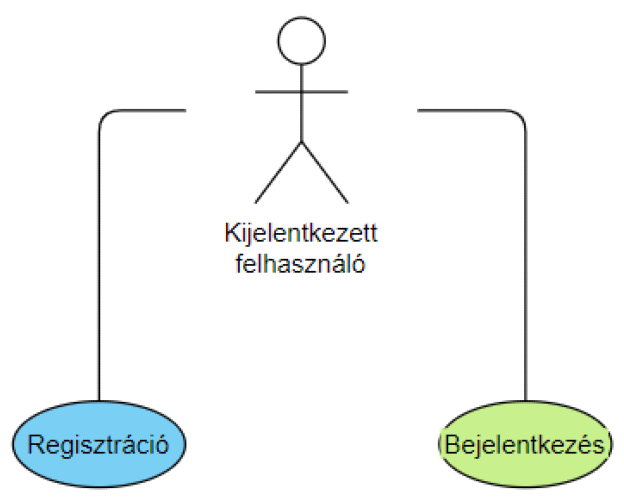
\includegraphics[width=5cm, height=4cm]{model_0}
	\caption{A nem bejelentkezett felhasználó use case diagrammja}
	\label{fig:picture}
\end{figure}

Regisztráció és bejelentkezés után megtekinthetjük a csoportokat, módosíthatjuk vagy törölhetjük a fiókunkat. A módosítások közé tartozik a név, profilkép vagy jelszó megváltoztatása.

\begin{figure}[H]
\centering
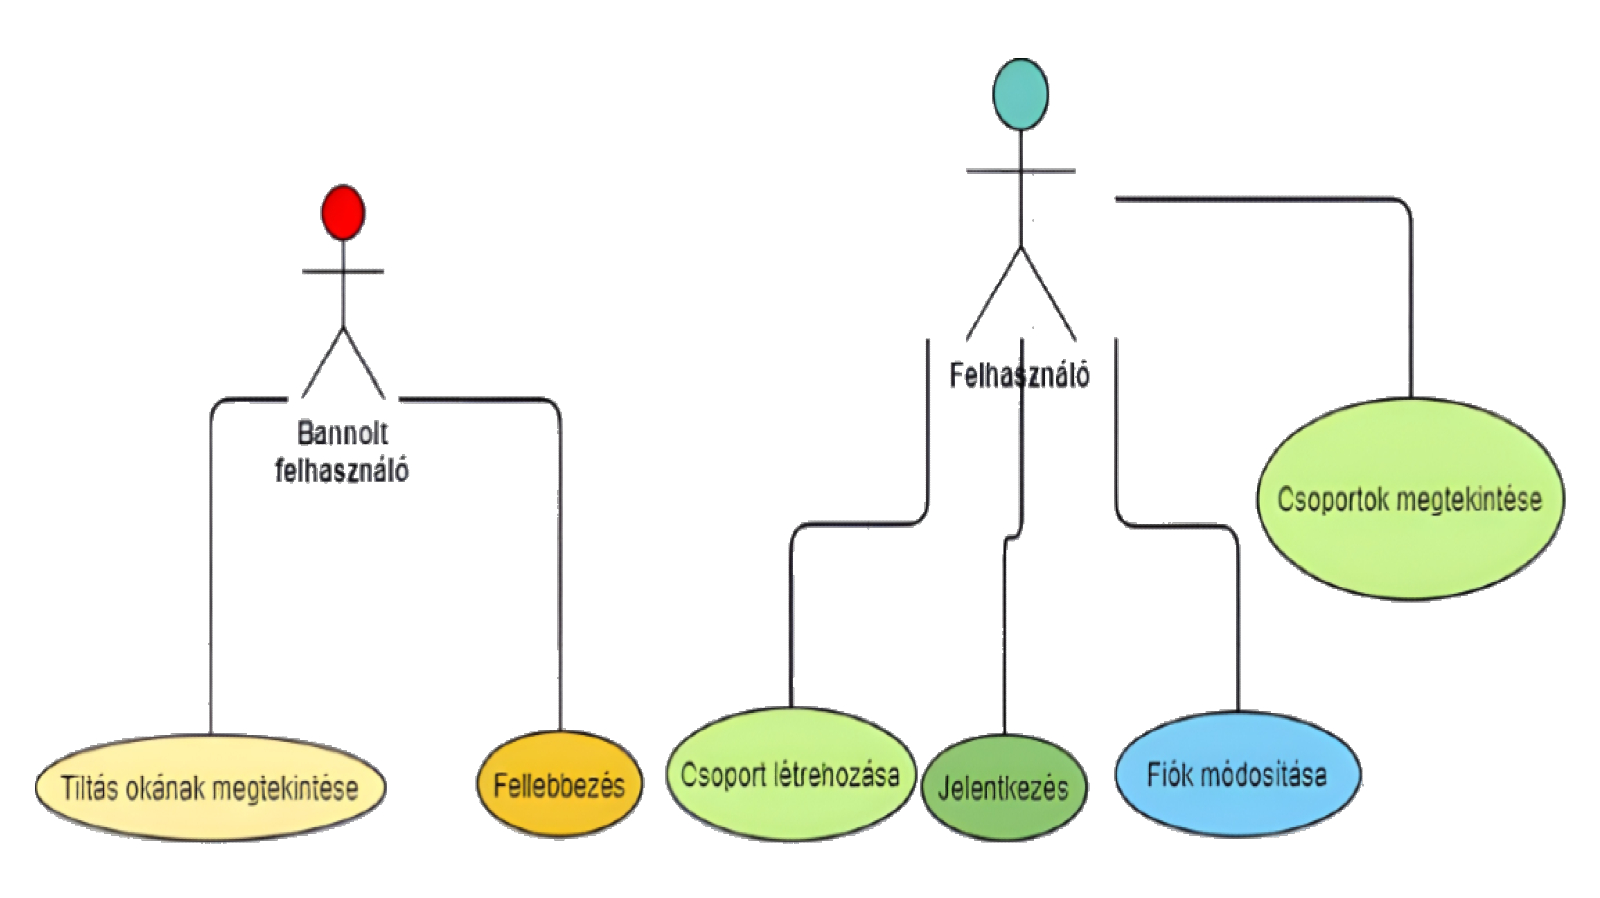
\includegraphics[width=14cm, height=5cm]{model_1}
\caption{A bejelentkezett és bannolt felhasználó use case diagrammja}
  \label{fig:picture}
\end{figure}

A fenti ábrán látható, hogy bejelentkezés után elérhetővé válik a fiókunk módosítása és törlése funkció, létre tudunk hozni csoportokat, vagy csatlakozhatunk meglévőkhöz, illetve kijelentkezhetünk. Moderátorként lehetőségünk van más felhasználók tartalmainak módosítására, vagy eltávolítására is. 

Abban az esetben, ha töröljük a felhasználónkat, még van lehetőségünk azt visszaállítani egy meghatározott ideig (egy hét). Ha egy admin tiltja a fiókunkat, akkor fellebbezhetünk és kérhetjük a fiók visszaállítását. Ha egy héten belül nem küldjük el a fellebbezést, akkor a tiltás végleges és a fiókunk automatikusan véglegesen törlődni fog az adatbázisból.
\pagebreak
\subsection{Követelménylista}

A következő táblázatban foglaltam össze a legfontosabb funkciókat, amiknek meg kell valósulniuk az alkalmazásban. Ezek közé tartozik az oldalak megtekintése, csoportok és posztok létrehozása, szerkesztése és törlése, a hozzászólás írása és a fellebbezés funkciók is.

\begin{table}[H]
	\begin{tabular}{|l|l|}
		\hline
		\rule{0pt}{4ex}\rule[-2ex]{0pt}{0pt}
		\textbf{Modul} &
		\textbf{Leírás}\\
		\hline
		Felhasználó létrehozása &
		\begin{tabular}[c]{@{}l@{}}
			Itt lehet új felhasználót létrehozni. Amennyiben már \\ létező felhasználót próbálunk létrehozni, vagy hibás \\ adatot adunk meg, hibaüzenetet kapunk.\end{tabular} \\
		\hline
		Autentikáció &
		\begin{tabular}[c]{@{}l@{}}
			Itt lehet bejelentkezni a fiókba megfelelő \\ felhasználónévvel és jelszóval. Amennyiben hibás adatot \\ adunk meg, hibaüzenetet kapunk.\end{tabular} \\
		\hline
		Név módosítása &
		\begin{tabular}[c]{@{}l@{}}
			Egy új felhasználónév megadásával módosíthatja a régit,\\ amennyiben az új név még nem foglalt.\end{tabular} \\
		\hline
		Jelszó módosítása &
		\begin{tabular}[c]{@{}l@{}}
			Először a régi jelszó megadásával hitelesíti magát a \\ felhasználó, majd az új jelszó megadásával módosíthatja \\ azt. Az új jelszót 2x kell megadni annak érdekében, hogy \\ a felhasználó ne zárja ki magát a fiókjából.\end{tabular} \\
		\hline
		Jogosultság &
		\begin{tabular}[c]{@{}l@{}}
		A következő szinteket kell létrehozni: vendég, tag, \\
		moderátor, admin.\end{tabular} \\ 
		\hline
		Csoport létrehozása &
		\begin{tabular}[c]{@{}l@{}}
			A csoport létrehozása funkció segítségével bárki saját \\ csoportokat tud létrehozni, melynek ő lesz az adminja.\end{tabular} \\
		\hline
		Tagság létrehozása &
		\begin{tabular}[c]{@{}l@{}}
			Itt tudnak a felhasználók csoportokhoz csatlakozni, \\
			A nyilvános csoportokba azonnal bekerülnek, míg a zárt \\ csoportokba csak egy admin vagy moderátor jóváhagyásával \\ kerülhetnek be.\end{tabular} \\
		\hline
		Csoport módosítása &
		\begin{tabular}[c]{@{}l@{}}
		A csoportadminok szerkeszthetik vagy törölhetik saját \\ csoportjaikat.\end{tabular} \\
		\hline
		\begin{tabular}[c]{@{}l@{}}Felhasználó oldal\\ Csoport oldal\\ Poszt oldal\end{tabular} &
		\begin{tabular}[c]{@{}l@{}}
			A felhasználók megtekinthetik a többi felhasználót, \\ csoportokat, posztokat és a posztokra érkezett megjegyzéseket. \end{tabular} \\
		\hline
		\begin{tabular}[c]{@{}l@{}}Tiltás és fellebbezés\end{tabular} &
		\begin{tabular}[c]{@{}l@{}}
			Az adminok törölhetik a nem helyén való tartalmakat. \\
			A tiltott felhasználóknak lehetőségük van megtekinteni \\
			a tiltás okát és fellebbezést indítani a tiltás ellen. \end{tabular} \\
		\hline
		\begin{tabular}[c]{@{}l@{}}Automatikus törlés\end{tabular} &
		\begin{tabular}[c]{@{}l@{}}
			Ha véletlenül törlünk valamit, azt még helyre lehet állítani \\
			egy adott ideig. Ha az idő letelik, a tartalom automatikusan \\
			törlődni fog az adatbázisból. \end{tabular} \\
		\hline
	\end{tabular}
\end{table}

\section{Funkcionális specifikáció}

\subsection{Célok}

Az alkalmazás célja, hogy a felhasználók ne egy platformtól függjenek, hanem kisebb csoportokat hozhassanak létre.

A felhasználók tematikus csoportokat hozhatnak létre, vagy már meglévőkhöz csatlakozhatnak és megoszthatják saját képeiket a többi hasonló érdeklődésű felhasználóval. A felhasználóknak lehetősége lesz törölni és szerkeszteni saját tartalmaikat, vagy mások tartalmaira reagálni egy hozzászólás írásával.

\subsection{Követelmények áttekintése}

Négy fő felhasználói szint van: az adminisztrátor, moderátor, tag és vendég.

\begin{figure}[H]
	\centering
	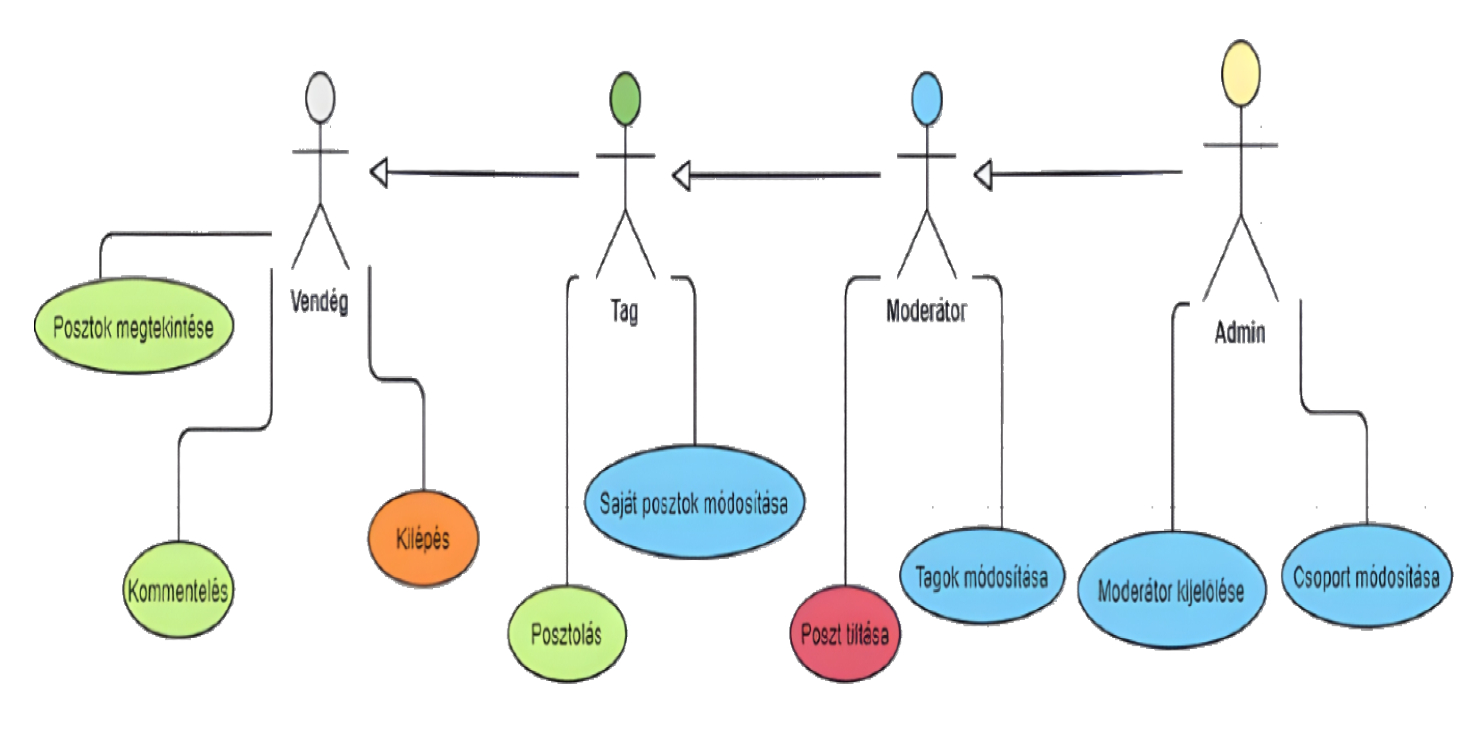
\includegraphics[width=15cm, height=5cm]{model_2}
	\caption{A csatlakozott felhasználók use case diagrammja}
	\label{fig:picture}
\end{figure}

A csoport tagok minden alattuk álló szerepkör képességeit megkapják. Például a moderátor tud posztolni és kommentelni is, mert ezeket egy tag is megteheti.

Ez azt is jelenti,  hogy egy moderátor csak a gyengébb szerepkörű felhasználókat módosíthatja, például egy vendégnek adhat tag szerepkört, de moderátor jogot már nem.

A vendégek meg tudják tekinteni a posztokat és írhatnak megjegyzéseket, de nem hozhatnak létre saját posztot. A tagok már létre hozhatnak saját posztokat és ezeket szabadon törölhetik vagy módosíthatják. A moderátorok már bárki posztját törölhetik a csoportból, és módosíthatják vagy törölhetik a csoport többi tagját. Az admin rendelkezhet az egész csoport felett, beállíthatja, a csatlakozás feltételeit, vagy a csoport láthatóságát. A csoport tulajdonosa törölheti, vagy szerkesztheti saját csoportját, illetve kioszthat moderátor és adminisztrátor jogosultságokat a tagok között.

\newpage 
\subsection{Képernyőtervek}

A funkciók megtervezése után meg kellett terveznem az alkalmazás megjelenését is. A következő képernyőtervek segítették a munkámat a frontend rész fejlesztésében.

\begin{figure}[H]
	\centering
	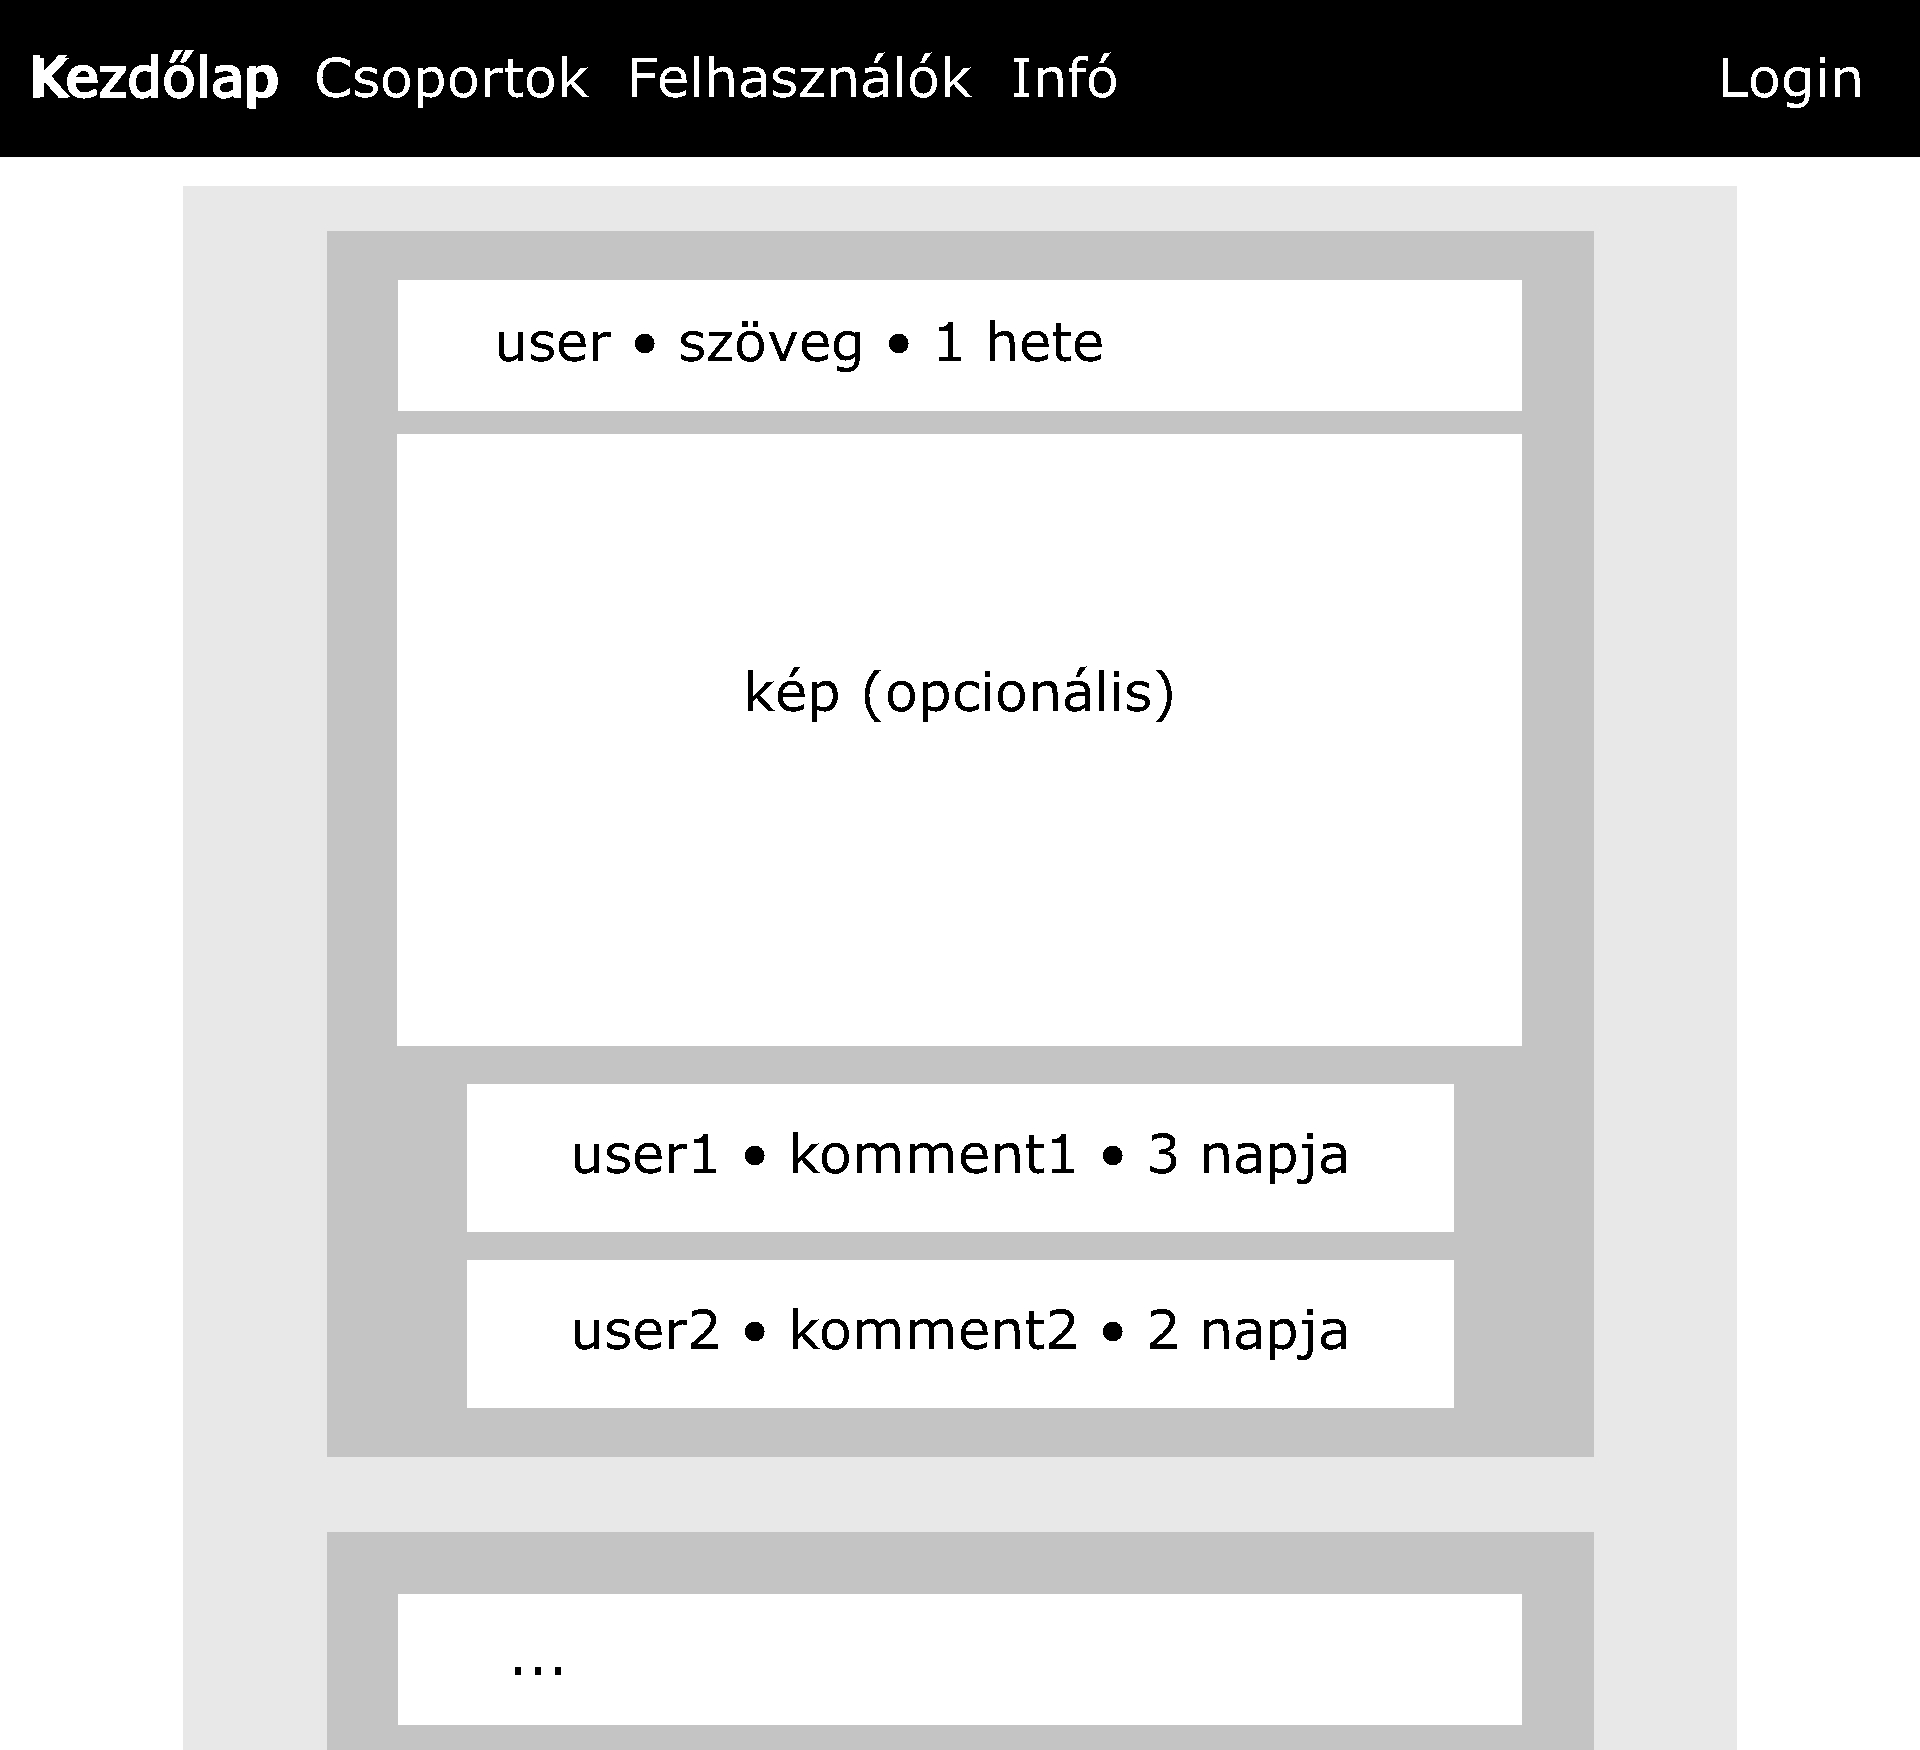
\includegraphics[width=12cm, height=6cm]{kepernyoterv1}
	\caption{A poszt oldal képernyőterve}
	\label{fig:picture}
\end{figure}

A csoport oldalon fognak megjelenni azok a posztok, amelyeket a többi tag osztott meg. Minden poszthoz tartozik egy egyedi URL, amit a poszt azonosítója határoz meg. Ezeket csak akkor láthatjuk, ha legalább vendég jogosultságunk van a csoportban. 

Azok a posztok nem jelennek meg, melyek törölve lettek, vagy privát láthatóságúak, kivéve abban az esetben, ha mi osztottuk meg őket.

Ha egy nem létező posztra hivatkozunk, vagy nincs jogosultságunk, akkor át leszünk irányítva egy hiba oldalra.

\begin{figure}[H]
	\centering
	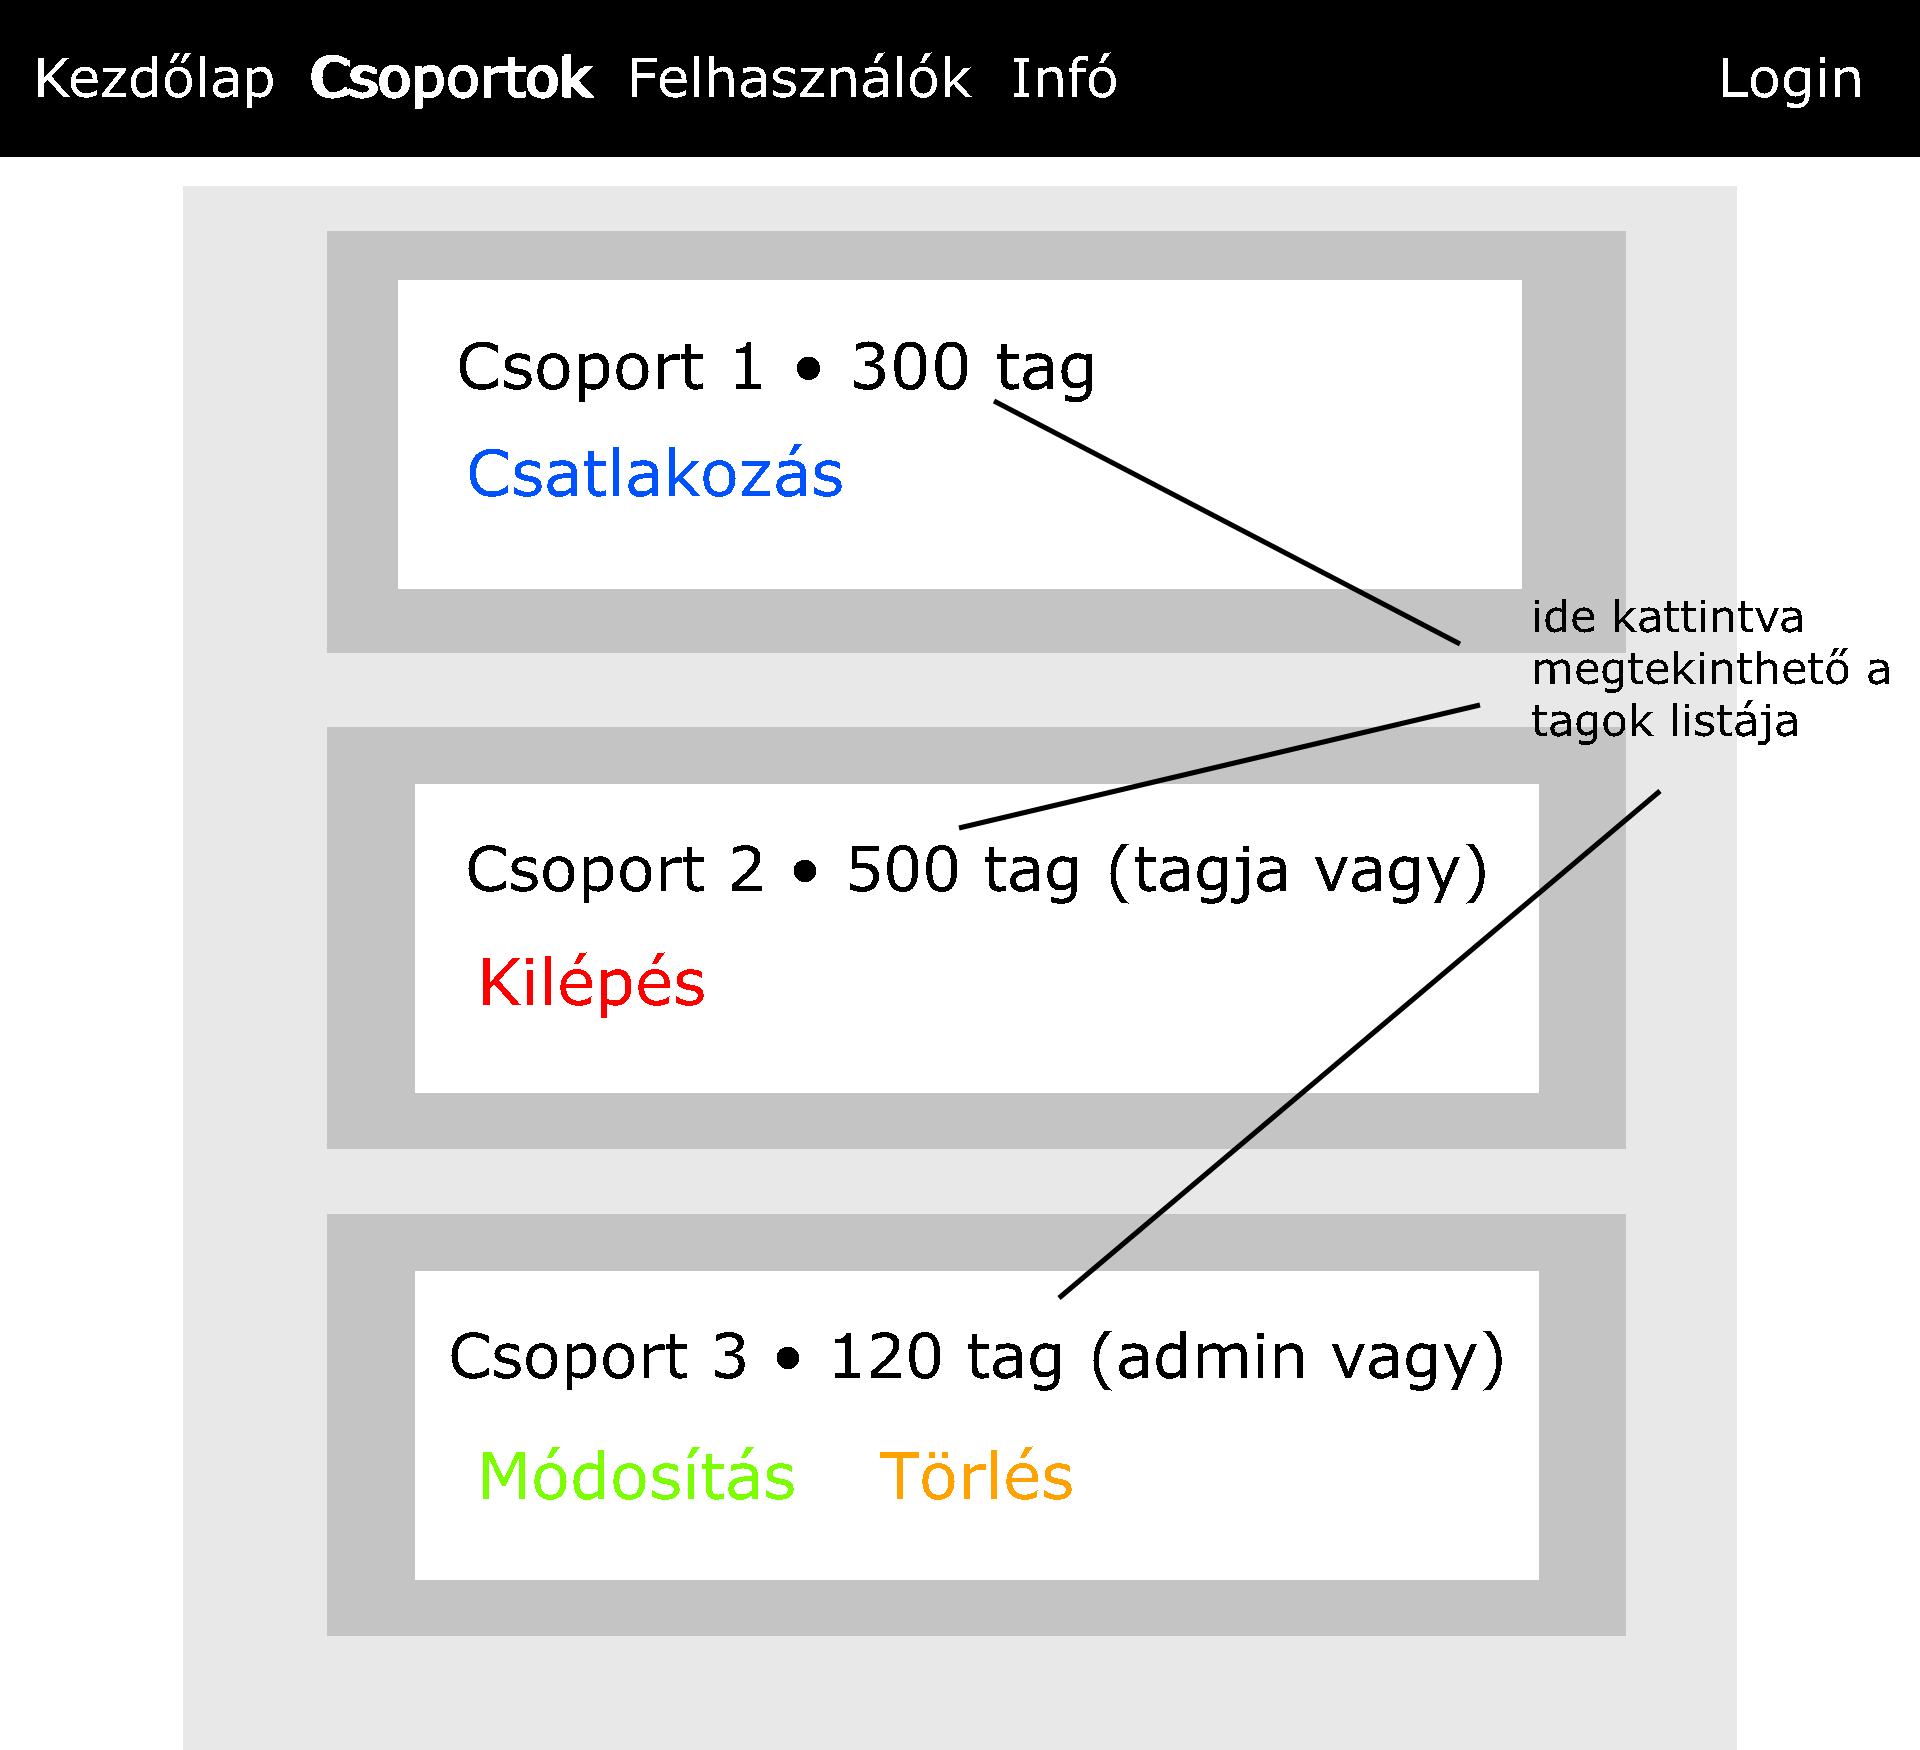
\includegraphics[width=12cm, height=6cm]{kepernyoterv2}
	\caption{A csoport lista oldal képernyőterve}
	\label{fig:picture}
\end{figure}

A "csoportok" fülre kattintva fognak megjelenni saját és a többi felhasználó által létrehozott nyilvános csoportok. Ha ezekre kattintunk, akkor, megtekinthetjük a posztokat. Abban az esetben, ha még nem vagyunk tagok, csak egy csatlakozás gomb jelenik meg.

\newpage 
\subsection{Forgatókönyvek}
\vspace{5mm}
\textbf{Regisztráció:} Meg kell adnunk egy legalább 5 karakter hosszú felhasználónevet és kétszer egy minimum 5 karakteres jelszót. Ha túl rövid jelszó vagy felhasználónév lett megadva, vagy már létező fiókot próbálunk regisztrálni, akkor hibaüzenetet kapunk. Ha a megadott jelszavak nem egyeznek, akkor is hibaüzenetet kapunk. Ha minden sikeres, az adatbázisban létrejön egy felhasználó és bejelentkezünk a fiókba. \\\\
\textbf{Bejelentkezés:} Egy felhasználónév - jelszó párral tudunk bejelentkezni. Ha a felhasználónévhez megfelelő jelszót adtunk meg, bejelentkezünk a fiókba, ellenkező esetben hibaüzenetet kapunk. \\\\
\textbf{Hozzáférés igénylése:} Ha egy csoportnak még nem vagyunk tagja, akkor kérhetünk hozzáférést. Egyes csoportokhoz automatikusan csatlakozhatunk, míg másokhoz csak admin jóváhagyásával férhetünk hozzá. \\\\
\textbf{Meghívás kezelése:} Ha meghívást kaptunk egy csoportba, akkor szabadon eldönthetjük, hogy elfogadjuk, vagy elutasítjuk. Abban az esetben, ha az "Elfogad" gombra kattintunk, hozzá leszünk adva a csoporthoz, míg az "Elutasít"-ra kattintva törölhetjük a meghívást az adatbázisból. \\\\
\textbf{Posztolás és hozzászólás:} Ha megkapjuk a tag rangot egy csoportban, akkor szabadon posztolhatunk. Ehhez meg kell adnunk egy szöveget és megadhatunk egy képet is, ha szeretnénk. Van lehetőségünk eldönteni, hogy posztunk megjelenjen-e a lista oldalon, vagy csak linkel legyen elérhető. A posztok közzétételét ütemezhetjük is egy jövőbeli dátum megadásával.\\\\
\textbf{Moderálás:} Moderátorként törölhetjük más felhasználók tartalmait a csoportból. Ehhez ki kell jelölnünk a tartalmat és meg kell adnunk egy indoklást. Azt is lehetőségünk van eldönteni, hogy csak a posztot töröljük-e, vagy a hozzá tartozó megjegyzéseket is. Azonos, vagy magasabb rangú felhasználók tartalmainál nem jelenik meg a tiltás lehetősége. \\\\

\section{Rendszerterv}

\subsection{Projekt terv}

A projekt egy közösségi média alkalmazás, ami PHP alapokon nyugszik. Ezek mellett HTML-t, CSS-t és JavaScript-et használok. Az adatbázis MySQL amit PhpMyAdmin segítségével hozok létre és XAMPP-on keresztül csatlakozok. Alkalmazásom részeit külön fejlesztem a fontosabb részekkel kezdve. Az ütemtervet és a feladatok kiosztását Trello-ban végzem, a verziókövetéshez SourceTree-t használok. 
\\\\
\textbf{A projekt ütemterve:}
\begin{enumerate}
	\item Alkalmazásötlet kialakítása, megtervezése
	\item A fejlesztőkörnyezetek kiválasztása, telepítése
	\item Ütemterv megírása
	\item Követelmények és funkciók specifikálása
	\item Rendszerterv létrehozása
	\item Adatbázis megtervezése és elkészítése
	\item Backend funkciók implementálása
	\item Felhasználói felület implementálása
	\item Tesztelés és véglegesítés
\end{enumerate}
\noindent
\textbf{Menük, gombok, menü hierarchiák:}
A menüben bejelentkezés előtt csak a Regisztráció és Bejelentkezés gombok lesznek láthatóak. Log-in után láthatjuk a Kezdőoldal, Csoportok és Felhasználók menügombokat, illetve a Profil gombot. Az utóbbira kattintva egy legördülő menüből érhető el a profilom oldal, ami a bejelentkezett felhasználó oldalára visz. Itt kap helyet egy Téma gomb, amivel a világos és sötét nézet között váltogathatunk. Ezeken kívül találunk itt egy Profil szerkesztése és egy kijelentkezés lehetőséget is.
\\\\
Abban az esetben, ha van jogosultságunk szerkeszteni valamit, megjelenik egy menü az adott objektum mellett. Ha ez a saját tartalmunk, akkor a menüből a Szerkesztés illetve a Törlés gombokat érhetjük el. Ha valaki más tartalmát van jogosultságom törölni, akkor csak egy Tiltás gomb jelenik meg.
\\\\
A csoportok oldalán 3 különböző gomb jelenhet meg: Belépés, Jelentkezés és Kilépés. Ha jóváhagyás nélkül jelentkezhetünk akkor a Belépés, ellenkező esetben a Jelentkezés gomb lesz elérhető. Ha már jelentkeztünk, akkor a kilépés gombot fogjuk csak látni.

\subsection{Fizikai környezet}

Ez a projekt egy webes alkalmazás lesz, amihez szükségünk van webszerverre és adatbázisra. Szerverünk a 80-as porton lesz elérhető. Az adatok egy MySQL adatbázisban lesznek tárolva, amit a PhpMyAdmin szolgáltatás segítségével könnyen el tudunk érni a \url{http://localhost/phpmyadmin} elérési úton. A kliens lehet bármely számítógép ami képes webböngészőt, például Google Chrome-ot futtatni. A fejlesztéshez Visual Studio Code-ot fogok használni Laravel keretrendszerrel. A megjelenéshez Bootstrap-et használok.

\subsection{Architekturális terv}

Az alkalmazás MVC-modellt (Model-View-Controller) használ. Az MVC egy architektúrális tervezési minta. Három fő rétegből áll: Model réteg, View réteg és Controller réteg.
\\\\
A \textbf{modell} rétegben található az adatbázis. Itt kapnak helyet az adatok, ez felel a tárolásukért és lekérdezésükért is. Itt találhatóak az adatokon módosításokat végző függvények is.

\lstinputlisting[caption=A poszt modelljének egy részlete,label=post.php]{codes/post.php}
\vspace{5mm}
A \textbf{nézet} réteg felel a felhasználói felület megjelenítéséért. Az adatok itt fognak megjelenni és ez fogja továbbítani a felhasználó által bevitt információkat a kontrollernek. A mi esetünkben itt kapnak helyet a blade.php fájlok.

Minden objektumtípusnál egy külön mappába tettem a megjelenítésért felelős fájlokat, mert egy oldal többféleképpen jelenhet meg. Például a ha egy törölt poszt URL-jét másoljuk a címsorba, akkor az annak megfelelő blade fájlt fogja betölteni.

\lstinputlisting[caption=Nem található komment oldal,label=404.blade.php]{codes/404.blade.php}
\vspace{5mm}

A \textbf{Kontroller} réteg felelős a vezérlésért. Itt kapnak helyet a kontroller osztályok. Ez fogja meghívni a nézeteket (blade fájlokat) a 'view' rétegben és a függvényeket a modell rétegben.

\lstinputlisting[caption=A "felhasználó profil oldal" nézetet meghívó kontroller függvény,label=controller.php]{codes/controller.php}
\vspace{5mm}

A 4-7 sorban található egy jogosultság ellenőrzés. Ez a legtöbb metódus előtt lefut, hogy megtudjuk, van-e jogunk az adott műveletet végrehajtani. A példában csak Log-in után tekinthetjük meg a profil oldalt és csak akkor, ha a fiókunk aktív. (vagyis nincs törölve, vagy tiltva)

Ezután lekérdezzük a megadott ID alapján az adatot. Ha nincs ilyen, akkor a kontroller meghívja a 404.blade.php nézetet. Utána lekérdezzük a megtekinteni kívánt felhasználó státuszát és meghívjuk a megfelelő nézetet. A státusz lehet aktív, törölt vagy tiltott. Csak akkor láthatjuk a tartalmat, ha az aktív.

\subsection{Adatbázis terv}

Az adatokat MySQL adatbázisban tároljuk, itt lesznek tárolva a felhasználók, a csoportok, a posztok, a hozzászólások és egyéb adatok, például a felhasználók jelentkezései.
Az adatbázis létrehozásához és szerkesztéséhez PhpMyAdmin szolgáltatást használok.
\\\\
\begin{figure}[H]
	\centering
	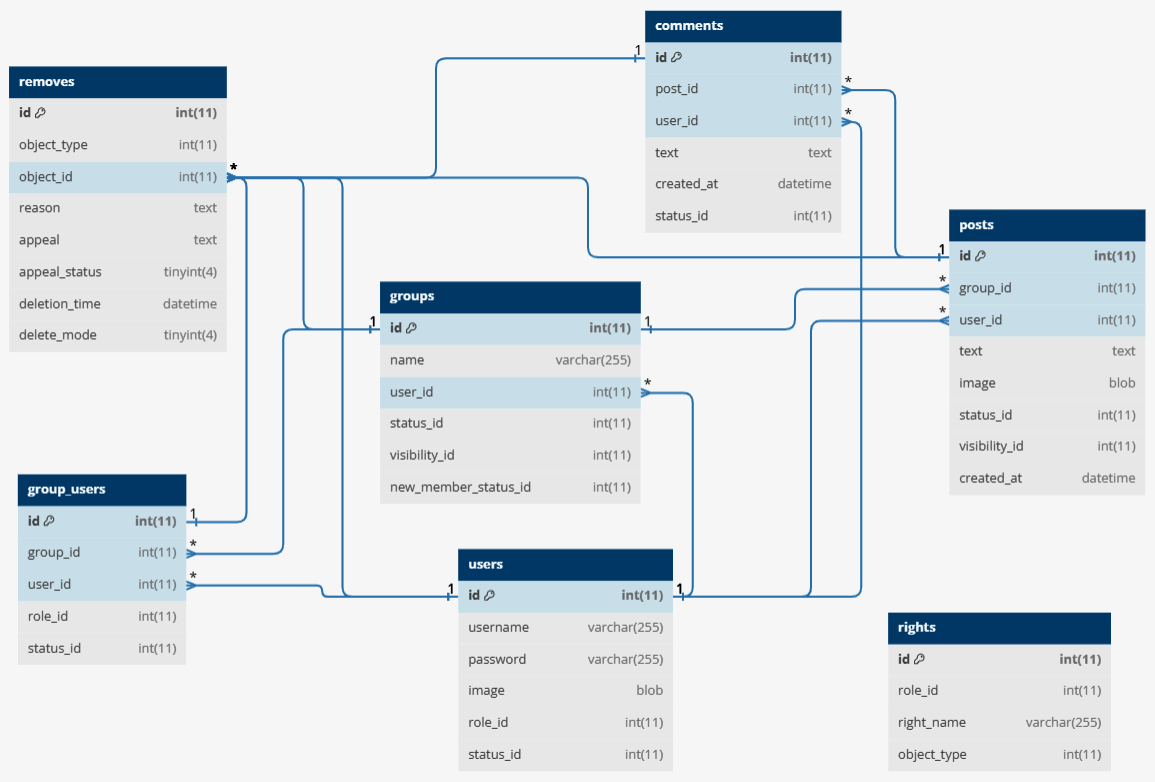
\includegraphics[width=15cm, height=10cm]{db}
	\caption{Az adatbázis fő táblái}
	\label{fig:picture}
\end{figure}
\pagebreak
\noindent
A \textbf{Csoportok} (Groups) Tábla:

\begin{table}[H]
	\begin{tabular}{|l|l|l|}
		\hline
		\rule{0pt}{4ex}\rule[-2ex]{0pt}{0pt}
		\textbf{Mező} &
		\textbf{Típus} &
		\textbf{Leírás} \\ 
		\hline
		ID &
		int &
		\begin{tabular}[c]{@{}l@{}}
			azonosító, elsődleges kulcs.\end{tabular} \\
		\hline
		name &
		varchar &
		\begin{tabular}[c]{@{}l@{}}
			csoport neve.\end{tabular} \\
		\hline
		user-id &
		int &
		\begin{tabular}[c]{@{}l@{}}
			csoport tulajdonosa.\end{tabular} \\
		\hline
		status-id &
		int &
		\begin{tabular}[c]{@{}l@{}}
			csoport státusza.\end{tabular} \\
		\hline
		visibility-id &
		int &
		\begin{tabular}[c]{@{}l@{}}
			csoport láthatósága. \end{tabular} \\
		\hline
		new-member-status-id &
		int &
		\begin{tabular}[c]{@{}l@{}}
			új tag státusza \end{tabular} \\
		\hline
		\end{tabular}
\end{table}
\noindent
Egy \textbf{csoport} létrehozásánál meg kell adnunk a \textit{nevét}, \textit{láthatóságát} és azt, hogy az új tagok azonnal, vagy csak jóváhagyás után csatlakozhatnak-e. A \textit{tulajdonos} automatikusan az lesz, aki létrehozta a csoportot. A \textit{státusz} alapértelmezés szerint "aktív" lesz.
\vspace{5mm}
\\
A \textbf{Felhasználók} (Users) Tábla:
\begin{table}[H]
	\begin{tabular}{|l|l|l|}
		\hline
		\rule{0pt}{4ex}\rule[-2ex]{0pt}{0pt}
		\textbf{Mező} &
		\textbf{Típus} &
		\textbf{Leírás} \\
		\hline
		ID &
		int &
		\begin{tabular}[c]{@{}l@{}}
			azonosító, elsődleges kulcs.\end{tabular} \\
		\hline
		username &
		varchar &
		\begin{tabular}[c]{@{}l@{}}
			egyedi felhasználónév.\end{tabular} \\
		\hline
		password &
		varchar &
		\begin{tabular}[c]{@{}l@{}}
			hash kódolt jelszó.\end{tabular} \\
		\hline
		image &
		blob &
		\begin{tabular}[c]{@{}l@{}}
			profilkép, opcionális.\end{tabular} \\
		\hline
		role-id &
		int &
		\begin{tabular}[c]{@{}l@{}}
			felhasználó szerepköre.\end{tabular} \\
		\hline
		status-id &
		int &
		\begin{tabular}[c]{@{}l@{}}
			felhasználó státusza. \end{tabular} \\
		\hline
	\end{tabular}
\end{table}
\noindent
Regisztráció után egy egyedi \textit{felhasználónév} és egy hash-elt \textit{jelszó} kerül az adatbázisba. A \textit{profilkép} alapértelmezés szerint NULL, de ezt később módosíthatjuk. Ha már van legalább 1 adminisztrátor szerepkörű felhasználó az adatbázisban, akkor a 'user' szerepkört kapjuk meg. Ellenkező esetben 'admin'-ként kerülünk az adatbázisba. A \textit{státusz} alapértelmezés szerint "aktív" lesz.
\vspace{5mm}
\\

\pagebreak
\noindent
A \textbf{Posztok} (Posts) Tábla:
\begin{table}[H]
	\begin{tabular}{|l|l|l|}
		\hline
		\rule{0pt}{4ex}\rule[-2ex]{0pt}{0pt}
		\textbf{Mező} &
		\textbf{Típus} &
		\textbf{Leírás} \\
		\hline
		ID &
		int &
		\begin{tabular}[c]{@{}l@{}}
			azonosító, elsődleges kulcs.\end{tabular} \\
		\hline
		group-id &
		int &
		\begin{tabular}[c]{@{}l@{}}
			poszt csoportja.\end{tabular} \\
		\hline
		user-id &
		int &
		\begin{tabular}[c]{@{}l@{}}
			poszt tulajdonosa.\end{tabular} \\
			\hline
		text &
		varchar &
		\begin{tabular}[c]{@{}l@{}}
			poszt szövege.\end{tabular} \\
		\hline
		image &
		blob &
		\begin{tabular}[c]{@{}l@{}}
			kép, opcionális.\end{tabular} \\
		\hline
		status-id &
		int &
		\begin{tabular}[c]{@{}l@{}}
			poszt státusza.\end{tabular} \\
		\hline
		visibility-id &
		int &
		\begin{tabular}[c]{@{}l@{}}
			poszt láthatósága. \end{tabular} \\
		\hline
		created-at &
		datetime &
		\begin{tabular}[c]{@{}l@{}}
			létrehozás ideje. \end{tabular} \\
		\hline
	\end{tabular}
\end{table}
\noindent
Posztolás után a kiválasztott csoport és a bejelentkezett felhasználó azonosítója automatikusan bekerül az adatbázisba. Ezen kívül meg kell adnunk egy szöveget és feltölthetünk egy képet is. A kép lehet akár gif formátumú is. Kiválaszthatjuk a poszt láthatóságát. Ha ütemezni szeretnénk, hogy mikor váljon elérhetővé a tartalmunk, akkor meg kell adnunk egy jövőbeli dátumot.
\vspace{5mm}
\\
A \textbf{Megjegyzések} (Comments) Tábla:
\begin{table}[H]
	\begin{tabular}{|l|l|l|}
		\hline
		\rule{0pt}{4ex}\rule[-2ex]{0pt}{0pt}
		\textbf{Mező} &
		\textbf{Típus} &
		\textbf{Leírás} \\
		\hline
		ID &
		int &
		\begin{tabular}[c]{@{}l@{}}
			azonosító, elsődleges kulcs.\end{tabular} \\
		\hline
		post-id &
		int &
		\begin{tabular}[c]{@{}l@{}}
			poszt, amire a komment érkezett.\end{tabular} \\
		\hline
		user-id &
		int &
		\begin{tabular}[c]{@{}l@{}}
			komment írója.\end{tabular} \\
		\hline
		text &
		varchar &
		\begin{tabular}[c]{@{}l@{}}
			komment szövege.\end{tabular} \\
		\hline
		status-id &
		int &
		\begin{tabular}[c]{@{}l@{}}
			komment státusza.\end{tabular} \\
		\hline
		created-at &
		datetime &
		\begin{tabular}[c]{@{}l@{}}
			létrehozás ideje. \end{tabular} \\
		\hline
	\end{tabular}
\end{table}
\noindent
A felhasználók hozzászólhatnak mások posztjaihoz. Ehhez csak egy szöveget kell megadni. A többi adat automatikusan lesz beállítva.
\vspace{5mm}
\\
\newpage
\noindent
A \textbf{Tagok} (Group-users) Tábla:
\begin{table}[H]
	\begin{tabular}{|l|l|l|}
		\hline
		\rule{0pt}{4ex}\rule[-2ex]{0pt}{0pt}
		\textbf{Mező} &
		\textbf{Típus} &
		\textbf{Leírás} \\
		\hline
		ID &
		int &
		\begin{tabular}[c]{@{}l@{}}
			azonosító, elsődleges kulcs.\end{tabular} \\
		\hline
		group-id &
		int &
		\begin{tabular}[c]{@{}l@{}}
			csoport, amibe a tag jelentkezett.\end{tabular} \\
		\hline
		user-id &
		int &
		\begin{tabular}[c]{@{}l@{}}
			jelentkezett felhasználó.\end{tabular} \\
		\hline
		role-id &
		int &
		\begin{tabular}[c]{@{}l@{}}
			tag szerepköre a csoporton belül.\end{tabular} \\
		\hline
		status-id &
		int &
		\begin{tabular}[c]{@{}l@{}}
			tagság állapota.\end{tabular} \\
		\hline
	\end{tabular}
\end{table}
\noindent
A \textbf{Group-user} tábla köti össze a felhasználókat a csoportokkal. Ha jelentkezünk egy csoportba, akkor a felhasználónk ID-ja és a csoport ID-ja kerül az adatbázisba. A szerepkörünk kezdetben 'Tag', a státuszunk pedig attól függ, hogy a csoport tulajdonos automatikus, vagy jóváhagyásos csatlakozást állított-e be.
\vspace{5mm}
\\
\noindent
A \textbf{Törlések} (Removes) Tábla:
\begin{table}[H]
	\begin{tabular}{|l|l|l|}
		\hline
		\rule{0pt}{4ex}\rule[-2ex]{0pt}{0pt}
		\textbf{Mező} &
		\textbf{Típus} &
		\textbf{Leírás} \\
		\hline
		ID &
		int &
		\begin{tabular}[c]{@{}l@{}}
			azonosító, elsődleges kulcs.\end{tabular} \\
		\hline
		object-type &
		int &
		\begin{tabular}[c]{@{}l@{}}
			törölt objektum típusa.\end{tabular} \\
		\hline
		object-id &
		int &
		\begin{tabular}[c]{@{}l@{}}
			törölt objektum azonosítója.\end{tabular} \\
		\hline
		reason &
		varchar &
		\begin{tabular}[c]{@{}l@{}}
			törlés indoklása.\end{tabular} \\
		\hline
		appeal &
		varchar &
		\begin{tabular}[c]{@{}l@{}}
			fellebbezés szövege.\end{tabular} \\
		\hline
		appeal-status &
		int &
		\begin{tabular}[c]{@{}l@{}}
			fellebbezés állapota.\end{tabular} \\
		\hline
		deletion-time &
		datetime &
		\begin{tabular}[c]{@{}l@{}}
			végleges automatikus törlés időpontja.\end{tabular} \\
		\hline
		delete-mode &
		int &
		\begin{tabular}[c]{@{}l@{}}
			törlés típusa.\end{tabular} \\
		\hline
	\end{tabular}
\end{table}
\noindent
Annak érdekében, hogy a törlés még visszaállítható legyen, minden objektumnak van egy 'status-id' nevű mezője. Ennek értéke lehet aktív, törölt vagy tiltott. Alapértelmezetten aktív, de ha töröljük valamelyik tartalmunkat, akkor az állapot 'Törölt' lesz. Megadhatjuk, hogy csak a kijelölt tartalmat, vagy a hozzá fűződő tartalmakat is törölni szeretnénk. Ha nem mi, hanem egy moderátor törli valamely tartalmunkat, akkor annak állapota 'Tiltott' lesz.

A törlést még visszaállíthatjuk, erre 1 hetünk van. Abban az esetben, ha tiltást kapunk, elolvashatjuk a tiltás okát, ami a 'reason' mezőben van eltárolva. Fellebbezésünket az 'appeal' mezőben tárolja a rendszer. Az 'appeal-status' mező tárolja, hogy elküldtük-e már a fellebbezést, vagy sem. Ha elküldünk egy fellebbezést, az egy hetes visszaszámlálás újraindul, és az admin-nak el kell fogadnia, vagy elutasítania a fellebbezést. Egy hét leteltével a rekord automatikusan törlődni fog a \textbf{removes} táblából.
\vspace{5mm}
\\
\noindent
A \textbf{Jogosultságok} (Rights) Tábla:
\begin{table}[H]
	\begin{tabular}{|l|l|l|}
		\hline
		\rule{0pt}{4ex}\rule[-2ex]{0pt}{0pt}
		\textbf{Mező} &
		\textbf{Típus} &
		\textbf{Leírás} \\
		\hline
		ID &
		int &
		\begin{tabular}[c]{@{}l@{}}
			azonosító, elsődleges kulcs.\end{tabular} \\
		\hline
		role-id &
		int &
		\begin{tabular}[c]{@{}l@{}}
			szerepkör, amivel a műveletet végrehajthatjuk.\end{tabular} \\
		\hline
		right-name &
		varchar &
		\begin{tabular}[c]{@{}l@{}}
			jogosultság megnevezése.\end{tabular} \\
		\hline
		object-type &
		int &
		\begin{tabular}[c]{@{}l@{}}
			objektum típusa, amin a \\ műveletet el akarjuk végezni.\end{tabular} \\
		\hline
	\end{tabular}
\end{table}
\noindent
Ebbe a táblába kerülnek a jogosultságok és szerepkörök, amivel rendelkeznünk kell a művelet elvégzéséhez. Moderátorként jogunk van mások tartalmát tiltani, de csak akkor, ha az "gyengébb" szerepkörű nálunk.

\vspace{5mm}
\noindent
\textbf{Egyéb táblák, kapcsolótáblák: }\\
\noindent
\\
Ezeknek a tábláknak a szerkezetük azonos, csak a tartalmuk különbözik. Egy \textbf{ID}-hoz egy \textbf{Név} tartozik.

\vspace{5mm}
\noindent
A \textbf{szerepkör} (roles) tábla tartalma:

\begin{table}[H]
	\begin{tabular}{|l|l|l|}
		\hline
		\rule{0pt}{4ex}\rule[-2ex]{0pt}{0pt}
		\textbf{ID} &
		\textbf{Név} &
		\textbf{Prioritás} \\
		\hline
		1 &
		Admin &
		4 \\
		\hline
		2 &
		Moderátor &
		3 \\
		\hline
		3 &
		Tag &
		2 \\
		\hline
		4 &
		Vendég &
		1 \\
		\hline
	\end{tabular}
\end{table}
\noindent
A prioritás mező fogja meghatározni, hogy mely szerepkörnek legyen hatalma a másik felett. Ha két felhasználónak azonos a prioritása, akkor egyiknek sem lesz jogosultsága módosítani a másikat.
\vspace{5mm}
\\

\pagebreak
\noindent
Az \textbf{állapotok} (status) tábla tartalma:

\begin{table}[H]
	\begin{tabular}{|l|l|}
		\hline
		\rule{0pt}{4ex}\rule[-2ex]{0pt}{0pt}
		\textbf{ID} &
		\textbf{Név} \\
		\hline
		1 &
		aktív \\
		\hline
		2 &
		törölt \\
		\hline
		3 &
		tiltott \\
		\hline
		4 &
		várólistás \\
		\hline
		5 &
		meghívott \\
		\hline
		6 &
		bannolt \\
		\hline
	\end{tabular}
\end{table}
\noindent
A 4-es, 5-ös és 6-os státuszok csak a group-user táblára vonatkoznak. Ha egy tagot kitiltunk valamely csoportból, akkor az 'tiltott' helyett 'bannolt' státuszt kap. Erre azért van szükség, mert a tiltásokat egy héten múlva törölné a rendszer, így bárki újra jelentkezhetne egy csoportba, ahonnan tiltva lett.
\vspace{5mm}
\\
\noindent
A \textbf{fellebbezés állapotok} (appeal-status) tábla tartalma:

\begin{table}[H]
	\begin{tabular}{|l|l|}
		\hline
		\rule{0pt}{4ex}\rule[-2ex]{0pt}{0pt}
		\textbf{ID} &
		\textbf{Név} \\
		\hline
		1 &
		nem elküldött \\
		\hline
		2 &
		elküldött \\
		\hline
		3 &
		elutasított \\
		\hline
		4 &
		elfogadott \\
		\hline
	\end{tabular}
\end{table}
\noindent
A fellebbezéseknek 4 állapotuk lehet. Abban az esetben, ha a tartalmunkat mi töröltük akkor a fellebbezés mező üresen marad, az 'appeal-status' mezőbe pedig a 4-es érték kerül. (ezért azt fellebbezés nélkül vissza tudjuk állítani)

Az 'elutasított' és 'elfogadott' értékek azért fontosak, hogy a felhasználó kapjon egy visszajelzést arról, hogy tartalma vissza lett-e állítva, vagy sem.
\vspace{5mm}
\\
\noindent
A \textbf{objektum típus} (object-type) tábla tartalma:

\begin{table}[H]
	\begin{tabular}{|l|l|}
		\hline
		\rule{0pt}{4ex}\rule[-2ex]{0pt}{0pt}
		\textbf{ID} &
		\textbf{Név} \\
		\hline
		1 &
		felhasználó \\
		\hline
		2 &
		poszt \\
		\hline
		3 &
		csoport \\
		\hline
		4 &
		tagság \\
		\hline
		5 &
		komment \\
		\hline
	\end{tabular}
\end{table}
\noindent
Mivel lehet 1-es ID-val rendelkező poszt és csoport is, ezért fontos, hogy egyértelműen hivatkozzunk a kijelölt objektumra. Nnem elég egy ID-t megadnunk, az objektum típusát is meg kell határoznunk. Ha például lekérdezzük a 2-es típusú 5-ös ID-val rendelkező objektumot, a rendszer egyértelműen tudni fogja, hogy mi az \textbf{5-ös} azonosítójú \textbf{poszt}-ra hivatkozunk.
\vspace{5mm}
\\
\noindent
A \textbf{Láthatóságok} (visibilities) tábla tartalma:

\begin{table}[H]
	\begin{tabular}{|l|l|}
		\hline
		\rule{0pt}{4ex}\rule[-2ex]{0pt}{0pt}
		\textbf{ID} &
		\textbf{Név} \\
		\hline
		1 &
		nyilvános \\
		\hline
		2 &
		nem listázott \\
		\hline
		3 &
		privát \\
		\hline
	\end{tabular}
\end{table}
\noindent
Beállíthatjuk, hogy kik lássák a tartalmainkat. Ha privátra állítjuk, akkor csak mi láthatjuk. Nem listázott beállítással posztunkat bárki megtekintheti, aki tagja a csoportnak és ismeri a poszt URL-jét. Nyilvános beállítással már meg fog jelenni posztunk a csoport főoldalán, azaz miden tag látni fogja.

Ezt nem csak posztoknál, hanem csoportoknál is beállíthatjuk. A privát csoportokba senki sem jelentkezhet, de meghívhatunk embereket, akik eldönthetik, hogy szeretnének-e csatlakozni.

\subsection{Implementációs terv}

Az alkalmazás PHP, HTML, CSS és Javascipt nyelven fog elkészülni. A különböző komponenseket külön rétegekre kell bontani. A modell rétegben kapnak helyet az adatok és a rajtuk műveleteket végző metódusok, a nézet (view) rétegben kapnak helyet a blade fájlok amelyek a felhasználói felület megjelenítéséért felelnek. A vezérlő (controller) rétegben kapnak helyet az alkalmazás irányításáért felelős funkciók.
\vspace{5mm}
\\
Elsőként a Regisztráció, bejelentkezés és kijelentkezés funkciókat implementálom. Ezután adom hozzá a felhasználó módosításával kapcsolatos opciókat, például a jelszó, vagy a profilkép módosítása lehetőséget.
Minden objektumtípushoz meg kell írnom a létrehozás, megtekintés, szerkesztés és törlés funkciókat.
\vspace{5mm}
\\
Következő lépéskén a csoportokat adom hozzá. Ez után következnek a tagságok, posztok és megjegyzések. A tagságokhoz meg kell írnom a csatlakozás, kilépés és új tag meghívása metódusokat.
\vspace{5mm}
\\
Végül módosítom a törlés lehetőséget, és soft delete-et vezetek be. Implementálom a fellebbezés és a visszaállítás funkciókat. Létrehozom az automatikus törlés funkciót.

\subsection{Telepítési terv}

Első lépésként egy webszervert fog kelleni, ehhez használhatunk XAMPP-ot, vagy Docker konténereket.

A klienshez egy böngészőt futtatni képes operációs rendszerre, például Windowsra és egy webböngészőre, például Google Chrome-ra lesz szükségünk.

Kelleni fog egy adatbázis szolgáltatás, ami támogatja a PHP nyelvet és a MySQL adatbázist. Ehhez én PhpMyAdmin-t használtam.

Ezután jöhet a Laravel keretrendszer telepítése és a forráskód, illetve az adatok importálása.

\subsection{Tesztelési terv}

Minél előbb érdemes elkezdeni tesztelni az alkalmazást, már a fejlesztés korai szakaszában. Érdemes a határesetekre koncentrálni, szándékosan hibás adatokat megadni, hogy kiderüljön, megfelelően működik-e a funkció.
\\\\
A manuális teszteléshez először készítettem egy listát, ahol felsoroltam azokat a komponenseket, modulokat, amelyeket érdemes letesztelni. Ezután végigmentem a projektem főbb funkcióin a tesztelési terv alapján. Ha hibákat találtam, azokat felírtam, majd javítás után újrakezdtem a tesztelést az első tesztlépéstől. Ez azért fontos, mert lehet, hogy a javítással elrontottam egy korábban működő funkciót.
\\\\
A teszteknél érdemes kipróbálni olyan lehetőségeket is, amire a felhasználó nem is gondolna. Ilyen lehet például egy hibás URL megadása, vagy a profilkép feltöltésnél valamilyen más típusú fájl feltöltése.
\\\\
Természetesen nincs kimerítő teszt, de megtalálhatjuk és javíthatjuk vele a hibákat. Fontos, hogy azokra a részekre koncentráljunk, ahol magas a hibák lehetősége. Egy részt érdemes többször többféleképpen is tesztelni, mert lehet, hogy bizonyos bemenetekre kapunk hibát, míg másokra nem.
\\\\
Minél több tesztet végzünk, annál jobban megbízhatunk a programunkban, de sosem lehetünk biztosak abban, hogy szoftverünk tökéletesen és hibátlanul működik.
\begin{table}[H]
	\centering
	\begin{tabular}{|l|l|l|}
		\hline
		\rule{0pt}{4ex}\rule[-2ex]{0pt}{0pt}
		\textbf{ID} &
		\textbf{Tesztlépés} &
		\textbf{Siker / Hibaüzenet} \\
		\hline
		1. &\begin{tabular}[c]{@{}l@{}}
			Az alkalmazás \\ megnyitása
		\end{tabular} &
		A program lefut, minden megfelelően megjelenik \\ \hline
		2. & 
		\begin{tabular}[c]{@{}l@{}}
			Regisztrációs oldal \\ megnyitása
		\end{tabular} &
		Az oldal megnyitható/elérhető \\ \hline
		3. & \begin{tabular}[c]{@{}l@{}}
			Regisztráció helyes \\ adatokkal
		\end{tabular} &
		A regisztráció sikeres \\ \hline
		4. & \begin{tabular}[c]{@{}l@{}}
			Regisztráció helytelen \\ adatokkal
		\end{tabular} &
		A hibaüzenet megjelenik, a regisztráció sikertelen \\ \hline
		5. & \begin{tabular}[c]{@{}l@{}}
			Létező felhasználó \\ regisztrálása
		\end{tabular} &
		A hibaüzenet megjelenik, a regisztráció sikertelen \\ \hline
		6. & \begin{tabular}[c]{@{}l@{}}
			Bejelentkezés oldal \\ megnyitása
		\end{tabular} &
		Az oldal megnyitható/elérhető \\ \hline
		7. & \begin{tabular}[c]{@{}l@{}}
			Bejelentkezés létező \\ felhasználóval
		\end{tabular} &
		A bejelentkezés sikeres \\ \hline
		8. & \begin{tabular}[c]{@{}l@{}}
			Bejelentkezés nem \\ létező felhasználóval
		\end{tabular} &
		A hibaüzenet megjelenik, a bejelentkezés sikertelen \\ \hline
		9. & \begin{tabular}[c]{@{}l@{}}
			Bejelentkezés hibás \\ jelszóval
		\end{tabular} &
		A hibaüzenet megjelenik \\ \hline
		10. & \begin{tabular}[c]{@{}l@{}}
			Kezdőlap oldal \\ megnyitása
		\end{tabular} &
		Az oldal minden tartalma megjelenik \\ \hline
		11. & \begin{tabular}[c]{@{}l@{}}
			Felhasználók oldal \\ megnyitása
		\end{tabular} &
		Az oldal minden tartalma megjelenik \\ \hline
		12. & \begin{tabular}[c]{@{}l@{}}
			Csoportok oldal \\ megnyitása
		\end{tabular} &
		Az oldal minden tartalma megjelenik \\ \hline
		13. &\begin{tabular}[c]{@{}l@{}}
			Kommentek, posztok, \\ csoportok kipróbálása
		\end{tabular} &
		\begin{tabular}[c]{@{}l@{}}
			Az objektumok létrehozhatóak, törölhetőek, \\ szerkeszthetőek
			és megtekinthetőek
		\end{tabular} \\
		 \hline
		14. & \begin{tabular}[c]{@{}l@{}}
			Kijelentkezés \\ tesztelése
		\end{tabular} &
		\begin{tabular}[c]{@{}l@{}}
			A felhasználó valóban kijelentkezett, csak a \\ regisztráció és log-in funkciók elérhetőek.
		\end{tabular} \\ \hline
		15. & \begin{tabular}[c]{@{}l@{}}
			Admin, moderátor \\ kipróbálása
		\end{tabular} &
		Módosíthat-e bárkit/bármit? \\ \hline
		16. & \begin{tabular}[c]{@{}l@{}}
			Láthatóság \\ tesztelése
		\end{tabular} &
		\begin{tabular}[c]{@{}l@{}}
			Nem láthatóak azok a tartalmak, amelyek \\
			megtekintéséhez nincs jogosultságunk
		\end{tabular} \\
		 \hline
		17. & \begin{tabular}[c]{@{}l@{}}
			Objektum \\ törlése
		\end{tabular} &
		A törölt objektum nem jelenik meg a listában \\ \hline
		18. &\begin{tabular}[c]{@{}l@{}}
			Menük tesztelése
		\end{tabular} &
		Minden megfelelően megjelenik, működik \\ \hline
		19. & \begin{tabular}[c]{@{}l@{}}
			Csatlakozás és \\ leiratkozás tesztelése
		\end{tabular} &
		\begin{tabular}[c]{@{}l@{}}
			A jelentkezés, meghívás és kilépés működik \\
			A jelentkezők befogadhatóak és kidobhatóak
		\end{tabular} \\ \hline
	\end{tabular}
\end{table}

\chapter{Telepítési útmutató}
\section{Bevezetés}
Ez a telepítési útmutató a Windows operációs rendszerű számítógépekre vonatkozik. Lehet, hogy a telepítés eltérhet más operációs rendszereken.
\\\\
Ebben a fejezetben fogom bemutatni, hogyan lehet a kész projektet telepíteni. Kétféle lehetőség van: telepíthetjük XAMPP, vagy Docker segítségével is.
\noindent
Első lépésként töltsük le a projektet a megadott github repository-ról:
\noindent
\vspace{3mm}
\\
\url{ https://github.com/benedeklazar/Szakdolgozat_HDMIJ3_2023}
\\
\vspace{2mm}
\\
\noindent
Ezután telepítsük a Composer-t a következő linkre kattintva:
\noindent
\vspace{3mm}
\\
\url{ https://getcomposer.org/download/}
\\
\vspace{2mm}
\\
\noindent
\textit{Előfordulhat, hogy a rendszer nem adja hozzá automatikusan a ComposerSetup/bin mappát a rendszerváltozókhoz. Ebben az esetben keressünk rá a start menüben "A rendszer környezeti változóinak módosítása"-ra és
a megjelenő ablakban kattintsunk a \textbf{Környezeti változók...} gombra.
A rendszerváltozóknál jelöljük ki a PATH nevűt és a szerkesztés gombra kattintva adjuk hozzá a ComposerSetup bin mappájának elérési útját. Ez alapértelmezetten a /Users/NÉV/AppData/Local/ComposerSetup mappában található.}
\\\\

\section{Projekt futtatása XAMPP-al}

Telepítsük a XAMPP-ot az Apache Friends weboldaláról. Használjuk a következő linket: \url{https://www.apachefriends.org/download.html}
\\
Nyissuk meg a XAMPP-ot, majd kattintsunk az Apache és MySQL modulok sorában a Start gombra.

\begin{figure}[H]
	\centering
	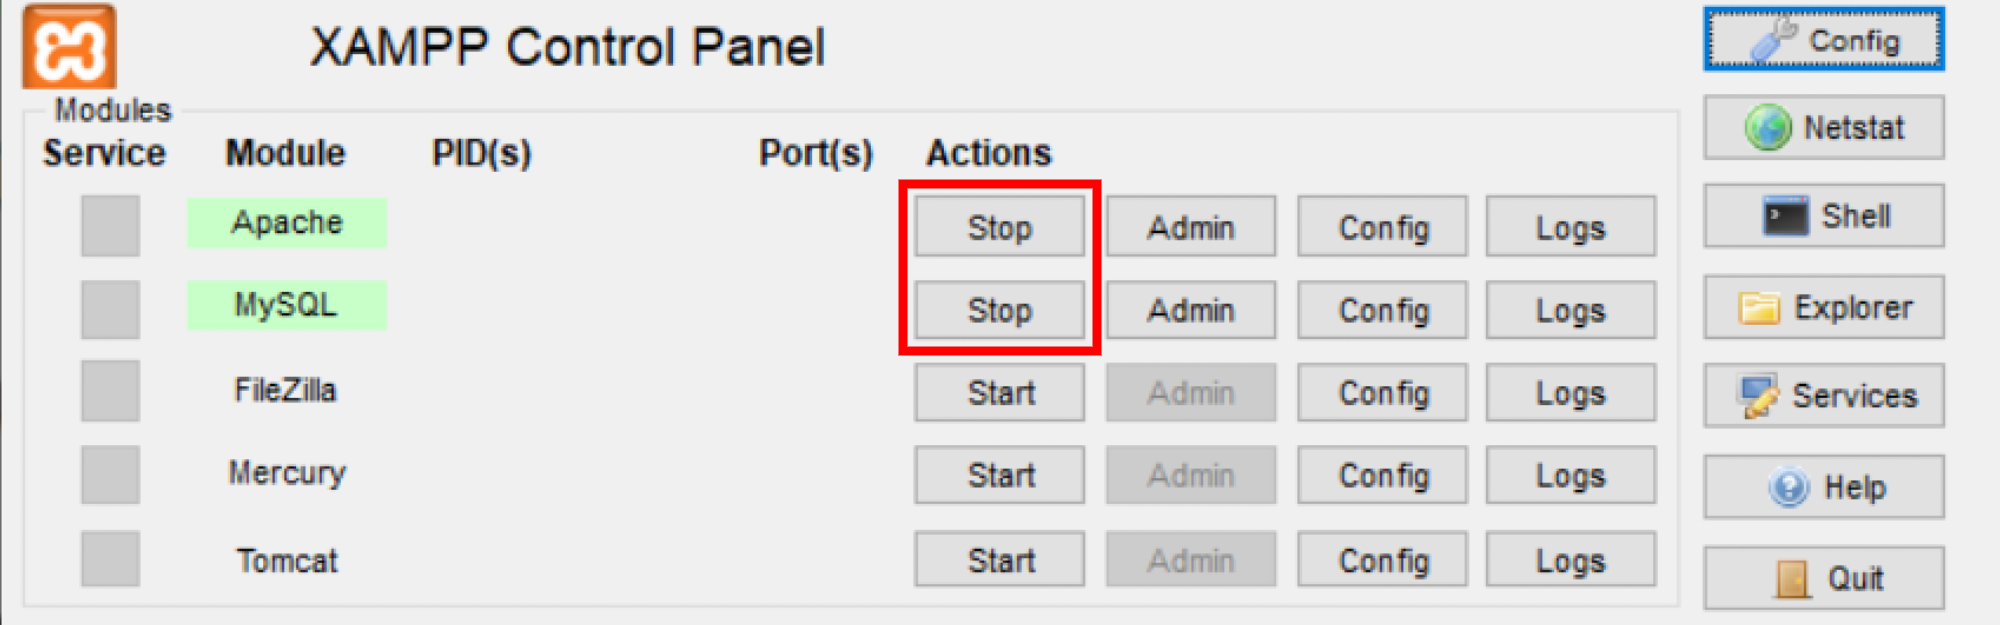
\includegraphics[width=13cm, height=5cm]{xampp}
	\caption{A XAMPP control panel}
	\label{fig:picture}
\end{figure}

Ha ezekkel megvagyunk, nyissuk meg a projektet és győződjünk meg róla, hogy a projekt gyökérmappájában vagyunk.
\\\\
Itt található egy start.ps1 nevű fájl. Az előkészítéshez ezt a fájlt kell futtatnunk. Ehhez írjuk be a parancssorba a következő powershell utasítást:
\\\\
\textbf{powershell -ExecutionPolicy Bypass -File start.ps1}
\\\\
Ezzel elindul a Composer telepítése. Ha mindent jól csináltunk, megjelenik a vendor mappa a navigációs ablakban. Ezután létrejön az .env fájl az .env\_2.example fájl alapján. Majd legenerálja az alkalmazás kulcsot és létrehozza az adatbázist. Következő lépésként futtatja a migrációkat, legenerálja a táblákat és feltölti alapértelmezett adatokkal. Végül elindítja az alkalmazást a 8000-es porton.
\\
Nyissuk meg a böngészőt és írjuk a címsorba következő linket, vagy kattintsunk ide: \url{http://localhost:8000/}
\begin{figure}[H]
	\centering
	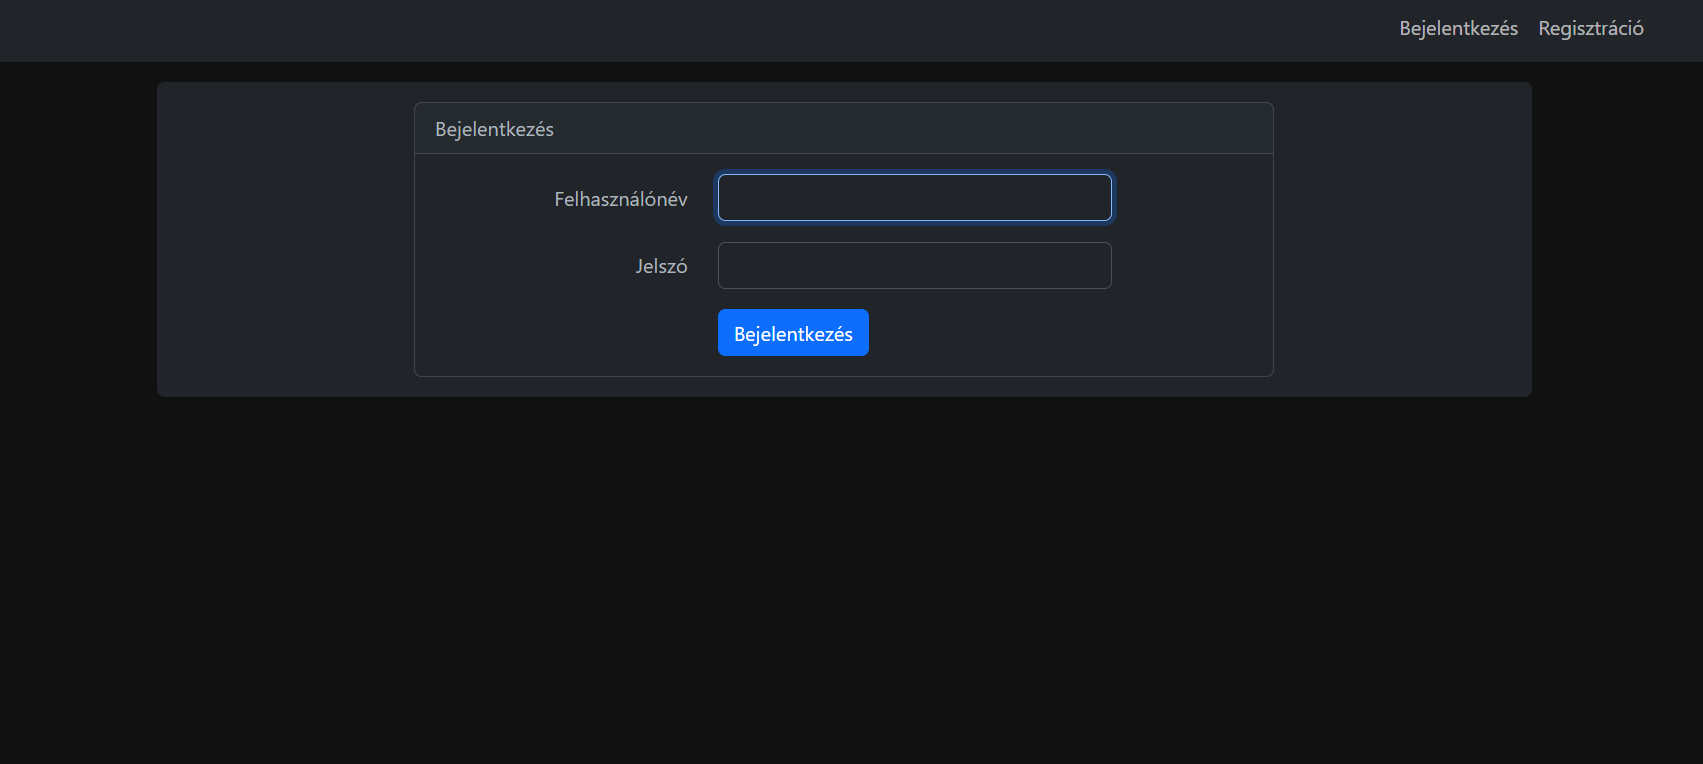
\includegraphics[width=13cm, height=7cm]{8000}
	\caption{Az alkalmazás nyitóoldala}
	\label{fig:picture}
\end{figure}
\noindent
Az alkalmazás nyitóoldala jelenik meg. Nézzük meg az adatbázist is, ehhez kövessük ezt a linket: \url{http://localhost/phpmyadmin/}
\\
Ha a generálás és migrációk futtatása során nem kaptunk hibát, itt találjuk a 'szakdolgozat\_hdmij3' nevű adatbázist, benne a táblákkal és kezdő adatokkal.

\section{Projekt futtatása Docker-rel}

Telepítsük a Docker desktop-ot a következő linkre kattintva:\\
\url{https://docs.docker.com/desktop/install/windows-install/}
\\\\
A telepítéshez szükség lesz linux kernel-re is. Ezt úgy érhetjük el, hogy a parancssorba begépeljük a \textbf{wsl --install} parancsot.
\\\\
Ezek után, nyissuk meg a projektet és ellenőrizzük, hogy a projekt gyökérmappájában vagyunk-e.
\\\\
Itt találunk egy docker.ps1 nevű fájl. Az előkészítéshez ezt a fájlt kell futtatnunk. Ehhez gépeljük be a terminálba a következő powershell parancsot:
\\\\
\textbf{powershell -ExecutionPolicy Bypass -File docker.ps1}
\\\\
Először létrejönnek a Docker konténerek, amelyek a docker-compose.yml fájlban lettek definiálva. Ezután lefut a Composer install, ha még nem létezne az autoload.php fájl a vendor mappában. Következő lépésként az .env fájl jön létre az .env.example fájl alapján. Majd legenerálja az app kulcsot és futtatja a migrációkat a 'php' nevű docker szolgáltatásban. Legvégül elindítja az alkalmazásunkat a 8000-es porton.
\\
Kattintsunk a következő linkre: \url{http://localhost:8000/}
\\
Az alkalmazás nyitóoldalán találjuk magunkat.
\begin{figure}[H]
	\centering
	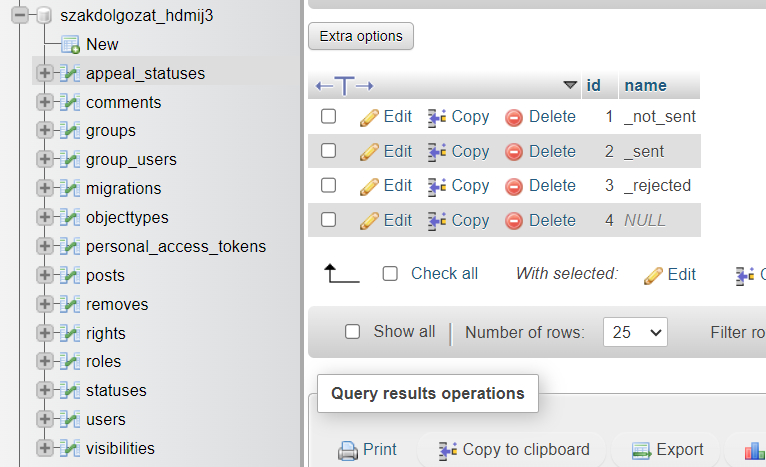
\includegraphics[width=15cm, height=8cm]{phpmyadmin}
	\caption{Az adatbázis PhpMyAdmin-ban}
	\label{fig:picture}
\end{figure}

A PhpMyAdmin szolgáltatás a 8090-es porton fog futni. \url{http://localhost:8090/}
\\
Először be kell jelentkeznünk. Az egyszerűség kedvéért a felhasználónév és a jelszó is '\textbf{root}'. Ezt megváltoztathatjuk az .env fájl módosításával.
\\\\
Sikeres bejelentkezés után láthatjuk az adatbázisunkat, táblákkal és adatokkal.

\chapter{Használt technológiák}
\section{Bevezetés}
Ebben a fejezetben fogom ismertetni azokat a technológiákat és szoftvereket, amelyeket a fejlesztés során használtam.
\section{Technológiák}

\subsection{XAMPP}

A XAMPP egy nyílt forráskódú szabad, platformfüggetlen webszerver. Főbb szolgáltatásai az Apache, a MySQL, a FileZilla, a Mercury és a Tomcat. A projekt adatbázisához és futtatásához csak az Apache és a MySQL szolgáltatásokat kell elindítani. A XAMPP egy betűszó, amely a következőt jelenti:

\begin{enumerate}
	\item \textbf{X} a platformfüggetlenséget jelenti
	\item \textbf{A}pache webszerver
	\item \textbf{M}ariaDB, vagy MySQL adatbázis
	\item \textbf{P}HP szerveroldali szkriptnyelv
	\item \textbf{P}erl általános célú szkriptnyelv
\end{enumerate}
\noindent
A XAMPP elérhetővé teszi a PhpMyAdmin szolgáltatást is, mely segítségével hoztam létre, és szerkesztettem az adatbázisom tábláit és mezőit.

\subsection{MySQL}

A MySQL egy nyílt forráskódú adatbázis kezelő rendszer, amely SQL nyelvet használ. Az SQL (Structured Query Language) egy strukturált lekérdezőnyelv, ami segítségével adatokat tudunk tárolni, lekérdezni, módosítani és törölni. A rendszer az adatokat táblákba rendezi. Ezeknek a tábláknak vannak oszlopaik, melyeket mezőknek, illetve soraik, melyeket rekordoknak nevezünk. Az eltárolt adatok gyakran összefüggnek egymással. Az adatok között lehet 1 az egyhez, egy a többhöz, és több a többhöz kapcsolat is.

\lstinputlisting[caption=A posztok táblát létrehozó kód SQL nyelven,label=sql.sql]{codes/sql.sql}
\vspace{5mm}

A .env fájlban adhatjuk meg, hogy milyen fajta adatbázist szeretnénk használni a projektünkhöz. A projektemben a DB\_CONNECTION változó értéke 'mysql'-re lett állítva.

\subsection{PhpMyAdmin}

A PhpMyAdmin egy adatbázis menedzsment eszköz, amit php nyelven írtak. Segítségével könnyen el lehet érni az adatbázisunkat és módosításokat tudunk rajta végrehajtani az interneten keresztül. Adatbázisokat és táblákat készíthetünk vele, a táblákat adatokkal tölthetjük fel.

A projekt adatbázisát itt hoztam létre, illetve a tesztelés során itt ellenőriztem, hogy egy adat sikeresen bekerült-e az adatbázisba, módosítva, vagy esetleg törölve lett.

\subsection{Laravel}

A laravel egy kifejezetten PHP webalkalmazások fejlesztését elősegítő keretrendszer, amely MVC (Model View Controller) tervezési mintát használ.
Sokat segít az adatbázis lekérdezések megírásában, hogy a fejlesztőknek azzal már ne kelljen foglalkozniuk. Továbbá készíthetünk alapértelmezett adatokat és migrációkat az adatbázisunkhoz.
A telepítés után létrejönnek a model, view és controller mappák, használhatjuk a blade sablonokat a nézet (view) rétegben, illetve az artisan parancsok is a rendelkezésünkre fognak állni.
Kapni fogunk egy 'routes' mappát, ahol felsorolhatjuk az alkalmazásunk linkjeit, és megadhatjuk, hogy mely metódusok legyenek meghívva.
Legenerálja az autentikációs és regisztrációs fájlokat, az 'auth' mappában, egy alapértelmezett bejelentkezési és regisztrációs oldallal.

\lstinputlisting[caption=A felhaználóhoz tartozó elérési utak,label=routes.php]{codes/routes.php}
\vspace{5mm}
\noindent
\\\\
A laravel egy jelenleg is bővülő keretrendszer, melyhez folyamatosan adnak hozzá újabb és újabb funkciókat. A Laravel weboldalán sok hasznos információval találkozhatunk, rengeteg példa kóddal és dokumentációval, amely akár a kezdő programozók számára is könnyen érthető. A dokumentációban minden fontos tudnivaló le van írva a keretrendszerről, megismerhetjük az adatbázis kezelést, a migrációk működését és leírásokat kapunk a beépített osztályok és metódusok használatáról, illetve működéséről is.
\\\\
A Laravel keretrendszer hivatalos dokumentációját a következő linkről érhetjük el:
\url{https://laravel.com/docs/10.x}

\subsection{CSS}

A CSS, vagyis Cascading Style Sheets (magyarul: "lépcsőzetes stíluslapok") egy stílusleíró nyelv, amely főként HTML dokumentumok megjelenését írja le. Ennek segítségével megadhatjuk a betűk színét, a háttérszínt, betűméretet, képek méretét és sok egyéb beállítást a kinézetre vonatkozóan.

\lstinputlisting[caption=Listaelem kijelölése sötét nézetben,label=css.php]{codes/css.php}
\vspace{5mm}

Az alkalmazásom több ilyen fájlt használ, hogy a listákat és menüket megfelelően megjelenítse. Ezekben a fájlokban van leírva, hogy ha az egérmutatót egy listaelem fölé viszem, akkor annak háttere legyen egy kicsit világosabb, vagy sötétebb a megadott témától függően. (Sötét nézetben világosabb, míg világos nézetben sötétebb lesz)
Külön blokkban van leírva a világos és sötét nézetre vonatkozó stílus. Ezek a stílusok vonatkoznak a listákra, és a legördülő menükben található listaelemekre is.
A css fájlokon kívül a blade fájlokban is meghatároztam stílusokat. Ezek csak a kijelölt HTML elemre fognak vonatkozni. Itt a 'class' tag-en belül meg kell adni egy egyedi nevet, a CSS fájlban pedig erre tudunk hivatkozni.

\subsection{Bootstrap}

A bootstrap egy frontend fejlesztőeszköz csomag, amely segítségével könnyen készíthetünk grafikai elemeket, például gombokat és űrlapokat weboldalunkhoz. HTML, CSS és JavaScript bővítményeket használ.

\begin{figure}[H]
	\centering
	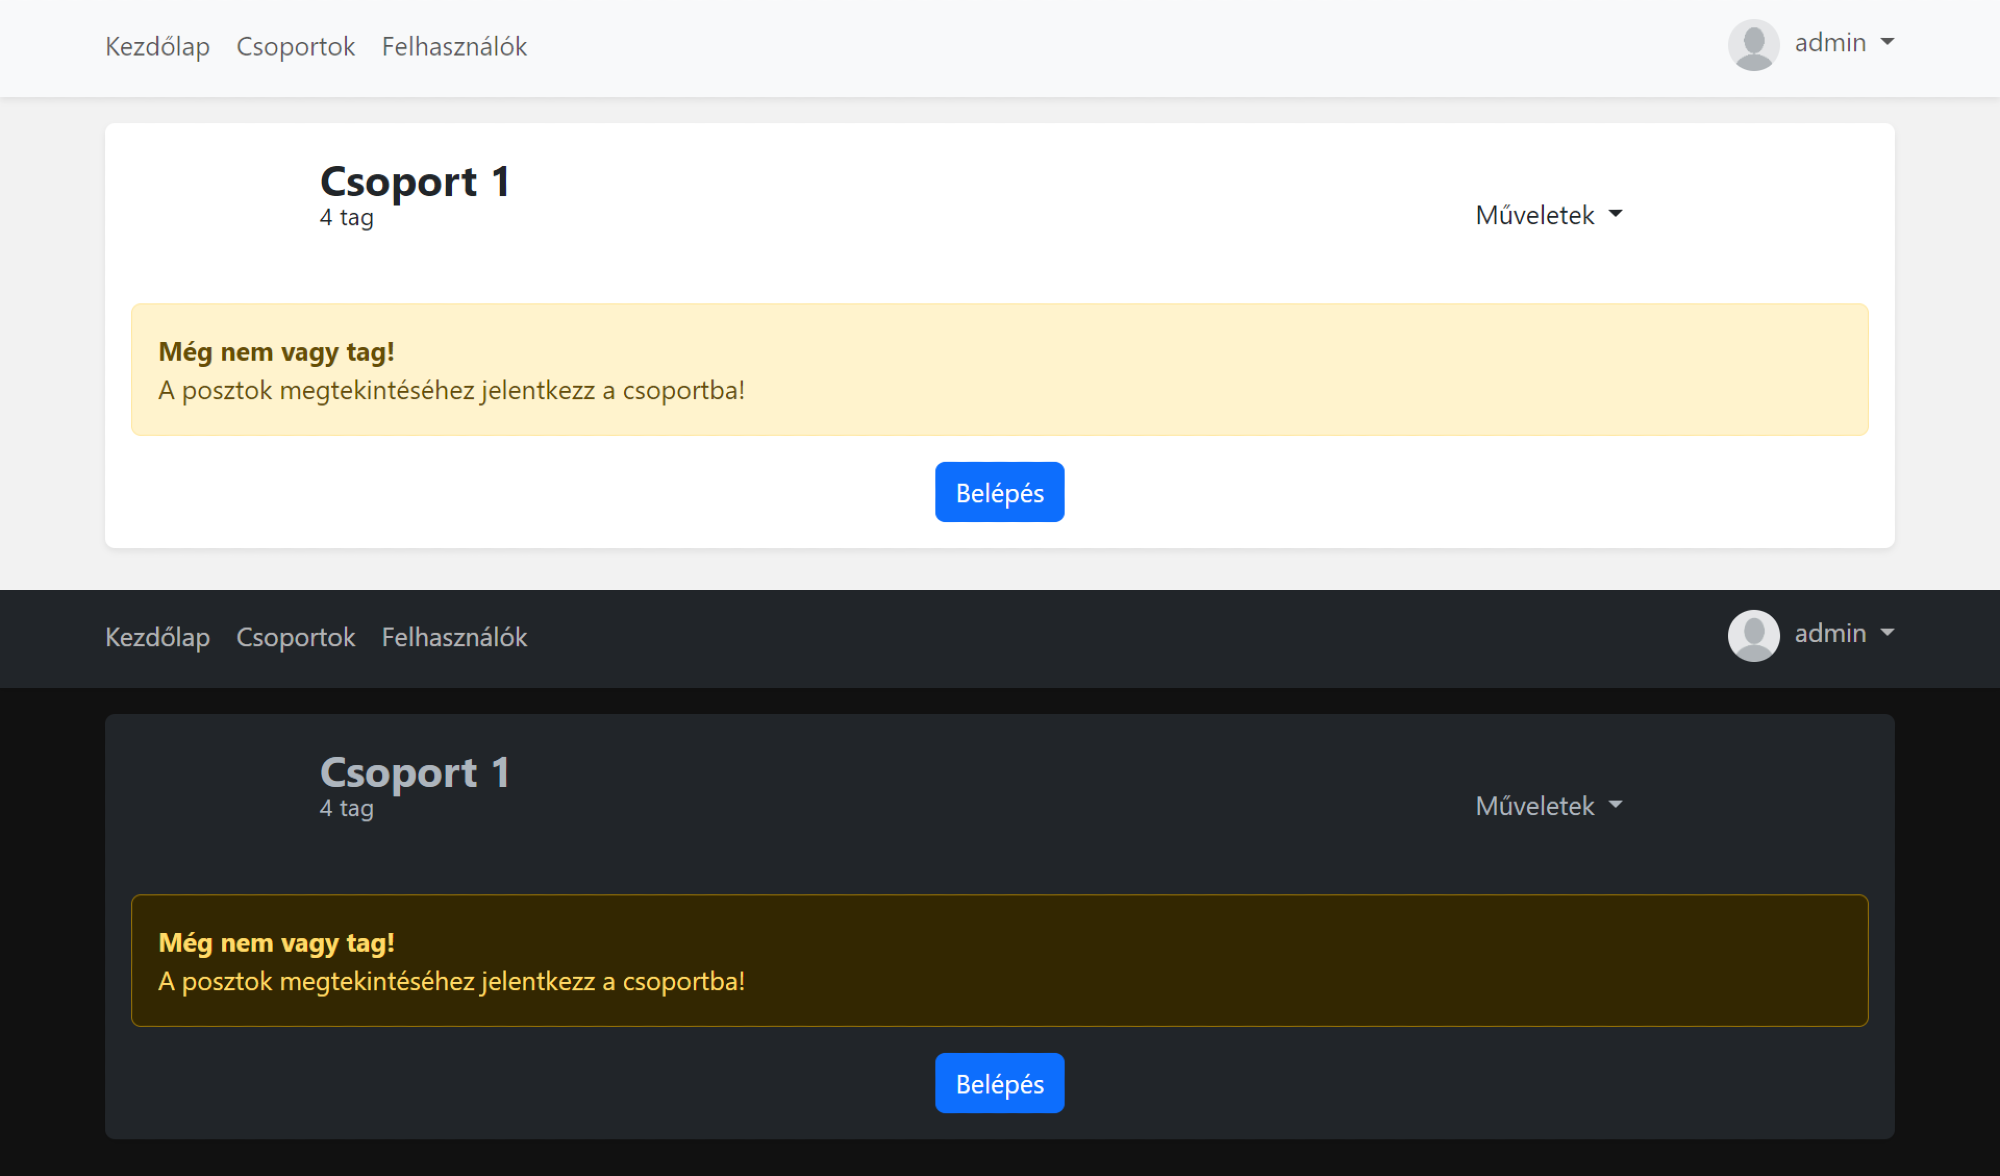
\includegraphics[width=15cm, height=8cm]{bootstrap}
	\caption{Bootstrap-el készült alert világos és sötét témával}
	\label{fig:picture}
\end{figure}
\noindent
Ha megnyitjuk az alkalmazást, az alapértelmezetten sötét lesz, de van lehetőségünk kiválasztani, hogy világos vagy sötét témával szeretnék-e használni. A beállításunkat menteni fogja a rendszer a böngésző sütijei között, ezért az addig érvényes marad, amíg meg nem változtatjuk.
\\\\
Ezen kívül van egy "Eszköz Témája" lehetőség is, amelyet, ha kiválasztunk, a rendszer automatikusan azt a témát fogja kiválasztani, amelyik a számítógépünkön alapértelmezett témaként van beállítva.
\\\\

\lstinputlisting[caption=A világos nézetet beállító JavaScript kód,label=light.php]{codes/light.php}
\vspace{5mm}

Ez a kód először a 'data-bs-theme' stílus osztály értékét világosra állítja, majd létrehoz egy 'theme' nevű változót a böngészőnk lokális tárhelyében, amit 'light' értékre állít.

Ha újratöltjük az oldalt, a data-bs-theme változó értékét a böngészőnkben elmentett értékre fogja állítani, amennyiben már van ilyen. Ha még nem állítottunk be stílust, a program a sötét témát fogja választani.

\section{Egyéb szoftverek és alkalmazások}
\subsection{SourceTree}

A SourceTree egy ingyenes Git kliens Windows és Mac rendszerekhez. A clone parancs segítségével feltölthetünk a számítógépünkön lévő projektet egy megadott GitHub repository-ba. Minden hozzáadott sort zölddel, míg a törölt sorokat pirossal fogja jelezni. 

\begin{figure}[H]
	\centering
	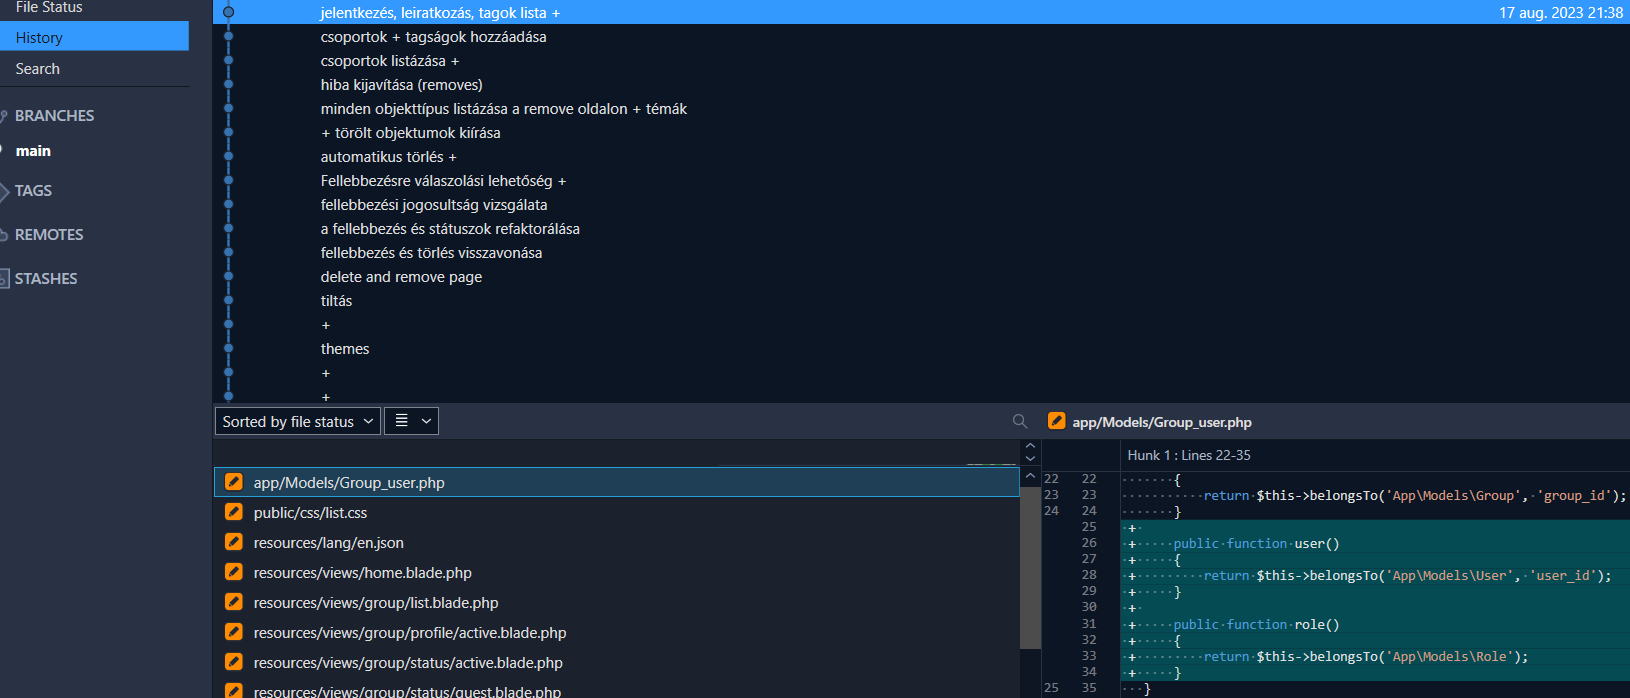
\includegraphics[width=15cm, height=8cm]{sourcetree}
	\caption{A SourceTree alkalmazás}
	\label{fig:picture}
\end{figure}
\noindent
A \textbf{'commit'} paranccsal a módosított és elmentett, de még fel nem töltött fájlok listáját tudjuk megtekinteni. Innen kiválaszthatjuk, hogy mely fájlokat szeretnénk végül feltölteni a GitHub-ra. A \textbf{'pull'} paranccsal a repository-ból tudjuk letölteni a fájlokat a lokális gépre, míg a \textbf{'push}' gomb megnyomásával a változtatások fognak felkerülni a repository-ra.
\\\\
A \textbf{'branch'}-el egy új ágat hozhatunk létre, ami hasznos, főleg ha többen dolgozunk egy projekten. Így a módosítások nem azonnal a main branch-re kerülnek, hanem egy saját ágra, amit a \textbf{'merge'} paranccsal vezethetünk vissza a fő ágba.

\subsection{Trello}

A trello egy kanban stílusú lista készítő webalkalmazás, ami a csoportos munkákat segíti elő. A felhasználók létrehozhatnak kártyákat, melyek egy-egy feladatot szimbolizálnak. Ezekhez hozzárendelhetnek egy felhasználót azaz azt a személyt, aki a feladatot kapta, és egy dátumot, ameddig azt teljesítenie kell.
\\\\
Segítségével a csapatok vizuálisan is láthatják, hogy éppen hol tart a projekt, melyek azok a feladatok, amelyek éppen folyamatban vannak.

\begin{figure}[H]
	\centering
	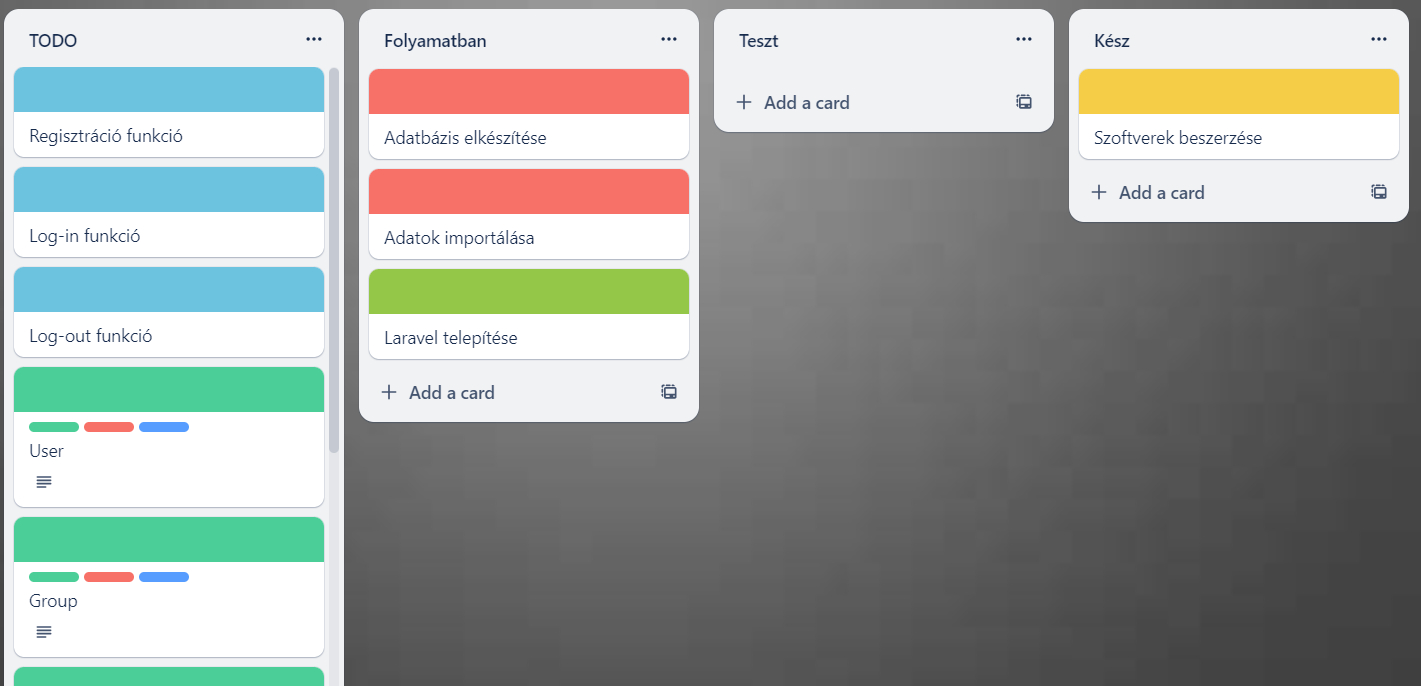
\includegraphics[width=15cm, height=8cm]{trello}
	\caption{A trello projekt oldala}
	\label{fig:picture}
\end{figure}

Tervezés után itt hoztam létre a követelménylistában szereplő feladatokat. Kezdetben nagyobb story-kat hoztam létre, melyeket később kisebb feladatokra (task-ekre) bontottam. Először a "TO-DO" (teendő) listából kiválasztottam egy feladatot, amelyet áthelyeztem a "Folyamatban" listára. Elkezdtem a rész kidolgozását, majd áthelyeztem a kártyát a "Teszt" oszlopba. Csak miután teljesen elkészítettem és leteszteltem egy részt, tettem a hozzá tartozó kártyát a "Kész" listába.

\subsection{Docker}

A Docker az egyik legnépszerűbb konténerizáló szoftver, amely képes operációs rendszer szintű virtualizációra. Ezzel kisebb szolgáltatásokat tudunk egy konténerbe csomagolni, egymástól elkülönítve.

\begin{figure}[H]
	\centering
	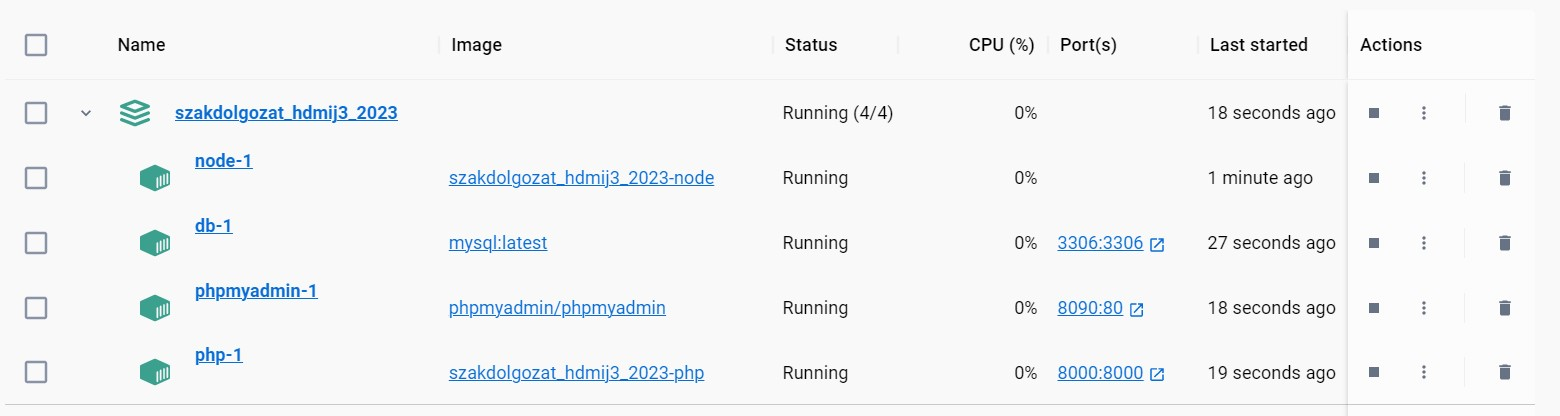
\includegraphics[width=15cm, height=5cm]{docker}
	\caption{A docker konténer a futó szolgáltatásokkal}
	\label{fig:picture}
\end{figure}

Az én webalkalmazásomban 4 ilyen elkülönített mikroszervíz van. A PHP, a MySQL, a Node és a PhpMyAdmin. A PHP szolgáltatáson keresztül fut a webszerver, a "db"-nek elnevezett MySQL-en pedig létrehozza az adatbázist a 3306-os porton. Az adatbázist a 8090-es porton lévő PhpMyAdmin szolgáltatással tudjuk elérni, illetve módosítani felhasználónév és jelszó megadását követően.

\chapter{Megvalósított funkciók}
\section{Bevezetés}
Ebben a fejezetben bemutatom az alkalmazásom főbb funkcióit és a működésüket. Ezeket a funkciókat a követelmény specifikációban található követelménylista alapján készítettem el. Minden metódus tartalmaz egy jogosultság ellenőrzést, hogy a felhasználók csak azokat a funkciókat használhassák, amelyek elérhetőek számukra. Ezután jön az adatok lekérdezése az adatbázisból. Végül a metódus megnyitja a megfelelő nézetet, vagy valamilyen adatbázis művelet után visszairányít minket az előző oldalra.

\section{Regisztráció és Bejelentkezés}

A Laravel egyik sajátossága, hogy a keretrendszer telepítésekor az autentikációs és regisztrációs funkciókat is legenerálja, ezért nekem csak néhány módosítást kellett ezeken végrehajtanom.

\lstinputlisting[caption=A regisztrációs adatok validálása,label=validate.php]{codes/validate.php}
\vspace{5mm}
\noindent
Regisztráció során egy legalább 5, maximum 255 karakter hosszú egyedi string-et kell megadni felhasználónévként, továbbá meg kell adnunk egy jelszót 2-szer, annak érdekében, hogy ne zárjuk ki magunkat egy elgépelés miatt. Ezeket a 'validator' nevű metódus ellenőrzi, és egy piros hibaüzenetet jelenít meg az űrlapon, ha valamely feltétel nem teljesül. A blade-ben minden input mezőhöz tartozik egy \textbf{@error} blokk, amiben egy alapértelmezett hibaüzenet fog megjelenni. Ezt módosítottam úgy, hogy a hibákat magyarul írja ki. Ehhez a 'resources' mappában található validation.php fájlt kellett módosítanom. Ennek segítségével akár több nyelvet is hozzáadhatunk a projektünkhöz.
\\\\
A bejelentkezés is hasonlóan működik. Ehhez meg kell adnunk a felhasználónevünket és a jelszavunkat. A rendszer megkeresi, hogy létezik-e felhasználó a megadott névvel az adatbázisban, majd ellenőrzi, hogy helyes jelszót adtunk-e meg. 
\lstinputlisting[caption=Az auth metódus,label=auth.php]{codes/auth.php}
\vspace{5mm}
\noindent
Az 'auth' metódus a bejelentkezett felhasználó egy paraméterben megadott tulajdonságával tér vissza. Például, ha a bejelentkezett felhasználó azonosítóját szeretnénk lekérdezni, a \$prop paraméternek 'id' értéket kell megadnunk.

\section{Profil oldalak}

A profil oldalak mindig egy azonosítót várnak, és egy nézettel térnek vissza, amennyiben van jogosultságunk annak megtekintéséhez. Nézzük meg mi történik, ha megnyitom a 'user/1' linket. Ilyenkor a UserController-ben lefut a profile metódus, amely 1-es értéket fog paraméterül kapni.
Jogosultság ellenőrzés után ellenőrzi, hogy létezik-e 1-es azonosítóval rendelkező felhasználó, és ha igen, akkor betölti a user.profile.active nézetet. (ha a felhasználó aktív)

\section{Létrehozás}

A létrehozáshoz szükségünk van egy 'create' és egy 'create\_form' metódusra. Néhány esetben meg kell adnunk egy paramétert is, például poszt létrehozásánál egy csoport azonosítót. Erre azért van szükség ,hogy tudjuk, a posztot mely csoportban szeretnénk megosztani.

A 'create\_form' metódus egy űrlap nézetet fog megnyitni, ahol megadhatjuk az új objektum adatait. A kész gomb megnyomása után lefut a 'create' metódus, amely az adatokat egy INSERT sql utasítással adja hozzá az adatbázishoz.

\section{Módosítás}

A módosításhoz 2 külön metódus kell. Egy (edit) ami megnyitja az űrlapot, ahol módosítani tudjuk az adatokat. Ezek GET módszert alkalmaznak. Ez azt jelenti, hogy az adatokat az URL-en keresztül adja át a metódusnak.
Itt nekünk csak egy azonosítót (például: 'user/edit/1') kell megadnunk, ezzel jelezve, hogy melyik adatot szeretnénk módosítani.

A másik metódus (update) fogja végrehajtani a módosításokat. Ez POST küldést használ és akkor fut le, amint megnyomjuk a 'Szerkesztés' gombot. A módosításokat egy \textbf{Request} típusú példányban adja át az 'update' metódusnak. Természetesen a kapott adatokat először validálni kell. Ha mindent rendben találtunk, lefut az UPDATE sql utasítás a megadott adatokkal.

\section{Törlés és Tiltás}

A törléshez és tiltáshoz meg kell adnunk a törölni kívánt objektum azonosítóját az URL-ben. A metódus ellenőrzi, hogy a megadott adatot van-e jogunk törölni. Törlés esetén azt vizsgálja, hogy a kijelölt objektum 'user\_id' mezőjében a bejelentkezett felhasználó azonosítója szerepel-e. Tiltás esetén azt ellenőrzi, hogy a bejelentkezett felhasználónak van-e Admin vagy Moderátor jogosultsága.

A törléshez és tiltáshoz is két-két külön metódust használtam. Egyet az űrlaphoz, és egyet az adatok módosításához. Az űrlapon meg lehet adni a törlés okát és módját. A 'submit' gomb megnyomása után a 'delete' metódusban valójában nem egy törlés, hanem egy létrehozás és egy módosítás megy végbe. Először létrehoz egy Remove rekordot, majd módosítja a törölni kívánt objektum státuszát töröltre.

\subsection{Automatikus törlés}

Az automatikus törlés a Remove táblában található delete\_time alapján történik. Először kilistázza az összes olyan rekordot, amely törlési ideje kisebb, mint a jelen időpont. Ezután Stratégia minta segítségével kiválasztja a megfelelő törlés metódust. Ezt a fellebbezések állapota alapján teszi meg. Abban az esetben, ha már küldtünk fellebbezést, és lejárt az idő anélkül, hogy választ kaptunk volna, az Appeal\_sent.php fájlban található auto\_delete metódus fog lefutni. Ilyenkor a tartalmunk automatikusan helyreáll, és a fellebbezés sikeresnek minősül.

\subsection{Törlési opciók}

Törlés létrehozásánál kiválaszthatjuk, hogy csak a kijelölt, vagy minden kapcsolódó tartalmat törölni szeretnénk-e. Ha csak a kijelölt objektumot töröljük, akkor a \$depth változó értéke 1 lesz. Ez határozza meg, hogy milyen mélységig fogjuk a tartalmakat törölni. Ha minden kapcsolódó tartalmat törlünk, akkor a 'delete' metódus rekurzívan fog lefutni, egészen addig, amíg el nem éri a megadott mélységet. Miután kigyűjtöttük a kapcsolódó tartalmakat, ugyanez a törlés metódus fog lefutni egyesével az összes ilyen objektumon, azzal a különbséggel, hogy a mélységet növeljük 1-el.

\section{Feliratkozás, leiratkozás}

A csoportokkal kapcsolatos főbb funkciók a Feliratkozás, Leiratkozás és Meghívás.
\\\\
Csatlakozásnál először azt ellenőrizzük, hogy a felhasználó tagja-e már a csoportnak. Ha már tagja, akkor ne legyen lehetősége újra csatlakozni.
Ezután megnézzük, hogy a csoport adminisztrátora engedélyezi-e a jelentkezést. Ha a 'new\_member\_status' mező értéke NULL, vagy a csoport láthatósága privát, akkor nincs lehetőségünk csatlakozni. Ha minden ellenőrzésen túljutottunk, akkor a felhasználó bekerül a csoportba, vagy felkerül a várólistára az admin beállításaitól függően.
\\\\
Ha várólistára kerültünk, meg kell várnunk az 'admiss' metódus futását. Ezt csak egy csoportadmin, vagy moderátor tudja meghívni. Ez a metódus egy várólistás tagot, aktív tagra fog módosítani.
\\\\
A meghívásnál csak egy űrlapot kell kitöltenie az adminnak, ahol megad egy olyan felhasználót, aki még nem tagja a csoportnak. Ezt a meghívott, az 'accept' metódus futtatásával tudja elfogadni. Ez a metódus akkor fut le, ha a csoport főoldalán megnyomjuk az \textbf{Elfogad} gombot.
\lstinputlisting[caption=A csatlakozás metódus,label=validate.php]{codes/join.php}
\vspace{5mm}
\noindent

\section{Jogosultságok kezelése}

Sok olyan metódus került az alkalmazásba, amit csak adminisztrátor, vagy moderátor tud használni. Ezek előtt a hasRight nevű metódus ellenőrzi, hogy van-e jogunk az adott művelethez. Ez a metódus mindig igazzal tér vissza, ha adminként, vagy a csoport tulajdonosaként vagyunk bejelentkezve. Ha ezek közül egyik sem igaz, akkor először összehasonlítja a szerepkörünket annak a felhasználónak a szerepkörével, aki birtokolja a megadott objektumot. Végül megnézi, hogy a Right táblában létezik-e a jogosultság és szerepkörünk elég magas-e a művelet elvégzéséhez. Ha magasabb rangúak vagyunk, mint a szerkeszteni kívánt objektum tulajdonosa és a rendszer megtalálta a jogot a Right táblában, a metódus TRUE-val tér vissza és szabadon szerkeszthetjük a kijelölt tartalmat.
\\\\
A metódusnak meg kell adnunk egy jogosultságot, és egy objektum típust és azonosítót. A típus és azonosító segítségével fogja megtalálni azt a tartalmat, amit módosítani, esetleg törölni szeretnénk. A jogosultságként egy szöveget adunk át, ezt fogja megkeresni a 'Right' táblában.

\section{Fellebbezés és helyreállítás}

Az alkalmazásom lehetőséget biztosít a felhasználóknak, hogy törölt tartalmaikat helyreállítsák. Ehhez egy űrlapot kell kitölteni, ahol megadják, hogy miért gondolják a tiltást tévesnek. Ez az űrlap egy POST küldéssel elmenti a fellebbezést az adatbázisban és a fellebbezés állapotát 'elküldött'-re módosítja. Ezen kívül az egy hetes visszaszámlálást újraindítja. Azt, hogy kinek legyen lehetősége fellebbezni, vagy fellebbezést elfogadni, az 'isDefendant' és 'isClaimant' metódusok fogják meghatározni. Az előbbi azt vizsgálja, hogy a bejelentkezett felhasználó tartalma lett-e törölve. Ha igen, akkor a kezdőoldalon megjelenik egy új listaelem, amely tartalmazza az eltávolított tartalmat, a fellebbezés állapotát és a végleges törlés idejét. Erre kattintva érjük el az űrlapot.
\\\\
Az isClaimant metódus fogja meghatározni, hogy ki az aki válaszolhat a fellebbezésünkre. Erre az 'admin' szerepkörű felhasználóknak van lehetőségük, feltéve, hogy a letiltott tartalom az ő csoportjukban lett megosztva.
\\\\
Mindkét metódus egy Remove rekord azonosítóját várja paraméterül. Ez az objektum típus és objektum azonosító mezők alapján visszakeresi a törölt objektumot, majd az isDefendant metódus esetén a 'user\_id'-t összehasonlítja a bejelentkezett felhasználóval, az isClaimant esetén pedig a 'group\_id' segítségével ellenőrzi, hogy a bejelentkezett felhasználónak van-e admin jogosultsága a csoportban. 

\chapter{Továbbfejlesztési lehetőségek}
\section{Bevezetés}
Egy alkalmazás sosincs kész, mert állandóan felmerülnek új felhasználói igények. Fontos, hogy bővíthető és rugalmas kódot írjunk, hogy ezeket az új igényeket könnyedén ki lehessen elégíteni. Ebben a fejezetben néhány olyan ötletet írok le, amivel az alkalmazásomat bővíteni lehet.

\section{Néhány bővítési lehetőség}

\textbf{Videók megosztása:} Az egyik ilyen lehetőség, hogy ne csak képeket, hanem videókat, vagy egyéb fájlokat is meg lehessen osztani. Ezzel a felhasználók több lehetőséget kapnak arra, hogy tartalmaikat megosszák másokkal.
\\\\
\textbf{Csoport szabályok:} Jelenleg egy admin eldöntheti, hogy az új tagok csak jóváhagyással csatlakozzanak. Ezt a funkciót bővíteni lehetne, hogy posztokra is vonatkozzon. Így a poszt privát maradna mindaddig, amíg azt egy admin jóvá nem hagyja.
\\\\
\textbf{Egyedi szerepkörök:} A csoporttulajdonosok kioszthatnának egyedi szerepköröket a meglévő admin, moderátor, tag és vendég szerepkörökön kívül, melyeknek megszabhatnák a jogait. Ezzel bővítenénk az adminok lehetőségeit.
\\\\
\textbf{Linkek, értesítések:} Poszt létrehozásánál a szövegben elhelyezhetnénk kattintható linkeket. Megjelölhetnék felhasználókat, akik értesítést is kapnak, vagy megoszthatnánk mások csoportjait. Ezzel a felhasználók könnyebben megtalálhatnák egymást.
\\\\
\textbf{Szövegek formázása:} A posztok és kommentek szövegét akár formázni is lehetne, ezzel kiemelve a fontosabb részeket. Hozzáadhatnánk kattintható linkeket, színezési lehetőséget, illetve félkövér és dőlt formázási lehetőségeket is.
\\\\
\textbf{Albumok:} Jelenleg csak egyesével tudunk képeket megosztani és ha új képet szeretnénk létrehozni, ahhoz egy külön posztot kell csinálnunk. Továbbfejlesztési lehetőségként egy posztban akár több képet is megoszthatnánk. Ezeket egy külön 'images' nevű táblában tárolnánk és a poszt azonosítójával hivatkoznánk a posztra. Több képhez is tartozhatna ugyanaz a poszt azonosító. 
\\\\
\textbf{Menü megjelenítése a profil oldalakon:} A profil oldalakon megjelenhetne minden olyan tartalom, melyet az adott felhasználó hozott létre. Egy menüből elérhetnénk az adott felhasználó által létrehozott csoportokat, posztokat és hozzászólásokat.


\chapter*{Összegzés}
\addcontentsline{toc}{chapter}{Összegzés}
Végezetül összegezzük, hogyan is készült el az alkalmazásom. Az ötletelés után megírtam a fejlesztői dokumentációt, kezdve a követelmény és funkcionális specifikációval. Majd létrejött a rendszerterv, ahol megterveztem az adatbázist és kiválogattam azokat a technológiákat, amelyeket használtam a fejlesztés során. Ezek után következett a keretrendszer telepítése, majd a programozás elkezdése.
Létrehoztam a tervezett funkciókat a követelménylista alapján. A fejlesztés közben gyakran teszteltem az alkalmazást, hogy biztos legyek abban, hogy mindent jól csináltam. Miután elkészült a projekt, a dokumentáció alapján még egyszer végigjártam a tesztlépéseket, és következhettek az utolsó simítások.
\\\\
Az első fejezetben ismertettem az adatbázis alapú webes alkalmazások főbb tulajdonságait. Olvashattunk a YouTube és a Facebook funkcióiról és az internet veszélyeiről is.
A második fejezetben láthattuk a dokumentációt, amely alapján elkészült az alkalmazás. Betekintést nyertünk az adatbázisba és láthattuk az alkalmazásom képernyőterveit és a megvalósítandó követelmények listáját is.
A harmadik fejezetben szó volt az alkalmazás telepítéséről. Lépésről-lépésre végighaladtunk a XAMPP-os és Docker-es telepítésen is.
A negyedik fejezetben részleteztem a felhasznált technológiákat, kezdve a MySQL-től, a Laravel-en át egészen a Docker-ig.
Ezt követően összegeztem az alkalmazásom főbb funkcióit és azok működését az ötödik fejezetben. Olvashattunk az automatikus törlésről és jogosultság ellenőrzésről is. Végül felsoroltam néhány továbbfejlesztési lehetőséget.
\\\\
Összességében ez a projekt sokat segített nekem abban, hogy jobban megismerkedjek a weboldalak fejlesztésével. Sokat tanulhattam a keretrendszerek, illetve az adatbázisok használatáról. Tapasztalatot szereztem a frontend fejlesztésben és dizájnolásban is a bootstrap-nek köszönhetően. Bele láthattam egy projekt menedzselésébe a Trello-val, és megismerkedtem a Docker konténerizációval is.

\chapter*{Köszönetnyilvánítás}

Szeretném köszönetet mondani az egyetemi tanáraimnak, elsősorban Dr. Tajti Tibor Gábor tanár úrnak, a sok hasznos tanácsért, a támogatásért és oktatásért, amely hozzájárult a szakdolgozatom létrejöttéhez és szakmai fejlődésemhez. Továbbá köszönetet mondok hallgatótársaimnak is, akik gyakran ötletekkel és útmutatással láttak el egyetemi éveim alatt.

\begin{thebibliography}{2}
\addcontentsline{toc}{chapter}{\bibname}
\bibitem{ProgTech}
\textsc{Dr. Kusper Gábor és Dr. Radványi Tibor}: \href{https://aries.ektf.hu/~hz/pdf-tamop/pdf-xx/ProgTechJegyzet.1.1.6.pdf}
{
	\emph{Jegyzet a projekt labor című tárgyhoz}
}, Eszterházy Károly Katolikus Egyetem, Eger, 2012.

\bibitem{ProgTech}
\textsc{Dr. Radványi Tibor}: \href{https://docplayer.hu/18547169-Adatbazisrendszerek-radvanyi-tibor.html}
{
	\emph{Adatbázisrendszerek}
}, 2014.

\bibitem{Internet useage}
\textsc{The World Bank}: \href{https://data.worldbank.org/indicator/IT.NET.USER.ZS}
{
	\emph{Az internethasználók százalékos aránya}
}

\bibitem{webapps wiki}
\textsc{Wikipedia}: \href{https://en.wikipedia.org/wiki/Web_application}
{
	\emph{Webalkalmazás}
}

\bibitem{adatbázis wiki}
\textsc{Wikipedia}: \href{https://hu.wikipedia.org/wiki/Adatb%C3%A1zis}
{
	\emph{Adatbázis}
}

\bibitem{közösségi média wiki}
\textsc{Wikipedia}: \href{https://hu.wikipedia.org/wiki/K%C3%B6z%C3%B6ss%C3%A9gi_m%C3%A9dia}
{
	\emph{Közösségi média}
}

\bibitem{facebook wiki}
\textsc{Wikipedia}: \href{https://hu.wikipedia.org/wiki/Facebook}
{
	\emph{Facebook}
}

\bibitem{youtube wiki}
\textsc{Wikipedia}: \href{https://hu.wikipedia.org/wiki/Youtube}
{
	\emph{YouTube}
}

\bibitem{twitter wiki}
\textsc{Wikipedia}: \href{https://hu.wikipedia.org/wiki/Twitter}
{
	\emph{Twitter}
}

\bibitem{XAMPP wiki}
\textsc{Wikipedia}: \href{https://hu.wikipedia.org/wiki/XAMPP}
{
	\emph{XAMPP}
}

\bibitem{XAMPP docs}
\textsc{Apache Friends}: \href{https://www.apachefriends.org/docs/}
{
	\emph{A XAMPP hivatalos dokumentációja}
}

\bibitem{MySQL wiki}
\textsc{Wikipedia}: \href{https://hu.wikipedia.org/wiki/MySQL}
{
	\emph{MySQL}
}

\bibitem{MySQL docs}
\textsc{MySQL}: \href{https://dev.mysql.com/doc/}
{
	\emph{A MySQL hivatalos dokumentációja}
}

\bibitem{PhpMyAdmin wiki}
\textsc{Wikipedia}: \href{https://hu.wikipedia.org/wiki/PhpMyAdmin}
{
	\emph{PhpMyAdmin}
}

\bibitem{PhpMyAdmin docs}
\textsc{PhpMyAdmin}: \href{https://www.phpmyadmin.net/docs/}
{
	\emph{A PhpMyAdmin hivatalos dokumentációja}
}

\bibitem{Laravel wiki}
\textsc{Wikipedia}: \href{https://en.wikipedia.org/wiki/Laravel}
{
	\emph{Laravel}
}

\bibitem{Laravel docs}
\textsc{Laravel}: \href{https://laravel.com/docs/10.x}
{
	\emph{A Laravel hivatalos dokumentációja}
}

\bibitem{CSS wiki}
\textsc{Wikipedia}: \href{https://hu.wikipedia.org/wiki/CSS}
{
	\emph{CSS}
}

\bibitem{CSS docs}
\textsc{W3SHOOLS}: \href{https://www.w3schools.com/css/default.asp}
{
	\emph{A CSS hivatalos dokumentációja}
}

\bibitem{Composer docs}
\textsc{Composer}: \href{https://getcomposer.org/doc/}
{
	\emph{A Composer hivatalos dokumentációja}
}

\bibitem{Bootstrap front-end framework wiki}
\textsc{Wikipedia}: \href{https://en.wikipedia.org/wiki/Bootstrap_(front-end_framework)}
{
	\emph{Bootstrap (front-end framework)}
}

\bibitem{Bootstrap docs}
\textsc{Bootstrap}: \href{https://getbootstrap.com/docs/5.3/getting-started/introduction/}
{
	\emph{A Bootstrap hivatalos dokumentációja}
}

\bibitem{SourceTree docs}
\textsc{Atlassian Documentation}: \href{https://confluence.atlassian.com/get-started-with-sourcetree}
{
	\emph{A SourceTree hivatalos dokumentációja}
}

\bibitem{Trello wiki}
\textsc{Wikipedia}: \href{https://hu.wikipedia.org/wiki/Trello}
{
	\emph{Trello}
}

\bibitem{Trello docs}
\textsc{Trello}: \href{https://trello.com/guide}
{
	\emph{A Trello hivatalos dokumentációja}
}

\bibitem{Kanban wiki}
\textsc{Wikipedia}: \href{https://hu.wikipedia.org/wiki/Kanban_(szoftverfejleszt%C3%A9s)}
{
	\emph{Kanban (szoftverfejlesztés)}
}

\bibitem{Docker docs}
\textsc{Docker Docs}: \href{https://docs.docker.com/}
{
	\emph{A Docker hivatalos dokumentációja}
}

\bibitem{Docker wiki}
\textsc{Wikipedia}: \href{https://hu.wikipedia.org/wiki/Docker_(szoftver)}
{
	\emph{Docker (szoftver)}
}

\bibitem{Docker hub}
\textsc{Docker Hub}: \href{https://hub.docker.com/}
{
	\emph{Docker Hub}
}

\bibitem{Koczka Ferenc}
\textsc{Koczka Ferenc}: \href{https://oprendszer.koczka.com/_static/kontenerek/kontenerek.html}
{
	\emph{Operációs Rendszerek, 16. Konténerek}
}

\bibitem{Emad Zaamout}
\textsc{YouTube - Emad Zaamout}: 
\href{https://www.youtube.com/watch?v=WahJ91Nrgn0}
{
	\emph{Laravel Docker Course | Complete Laravel Dockerization}
}

\bibitem{Kép feltöltése}
\textsc{CodeSource}: 
\href{https://codesource.io/complete-laravel-8-image-upload-tutorial-with-example/}
{
	\emph{Complete Laravel 10 Image upload Tutorial with an example}
}

\bibitem{A use case diagramokhoz használt Eszköz}
\textsc{Visual Paradigm}: 
\href{https://online.visual-paradigm.com/diagrams/features/use-case-diagram-software/}
{
	\emph{Use case diagram software}
}

\bibitem{Az adatbázis diagramokhoz használt Eszköz}
\textsc{DBDiagram.io}: 
\href{https://dbdiagram.io/d}
{
	\emph{Database Relationship Diagrams Design Tool}
}

\bibitem{Táblák generálásához használt Eszköz}
\textsc{Tables Generator}: 
\href{https://www.tablesgenerator.com/}
{
	\emph{HTML \& LaTeX table generator}
}

\bibitem{Képek és ikonok készítéséhez használt Eszköz}
\textsc{Pixlr X}: 
\href{https://pixlr.com/x/}
{
	\emph{Picture Editor}
}

\bibitem{Felhasznált betűtípus}
\textsc{Felhasznált betűtípus - Google Font}: 
\href{https://fonts.googleapis.com/css?family=Nunito}
{
	\emph{Nunito}
}

\bibitem{Felhasznált bootstrap stílus}
\textsc{Felhasznált bootstrap stílus}: 
\href{https://cdn.jsdelivr.net/npm/bootstrap@5.3.0/dist/css/bootstrap.min.css}
{
	\emph{bootstrap min 5.3.0 stylesheet}
}

\bibitem{Felhasznált bootstrap stílus}
\textsc{Felhasznált bootstrap stílus}: 
\href{https://cdn.jsdelivr.net/npm/bootstrap-icons@1.3.0/font/bootstrap-icons.css}
{
	\emph{bootstrap icons 1.3.0 stylesheet}
}

\bibitem{Latex}
\textsc{Dr. Tómács Tibor}: 
\href{https://tomacstibor.uni-eszterhazy.hu/latex.html}
{
	\emph{LaTeX – Számítógépes szöveg- és kiadványszerkesztés}
}


\end{thebibliography}

% Aláírt, szkennelt nyilatkozat beillesztése a szakdolgozat végére
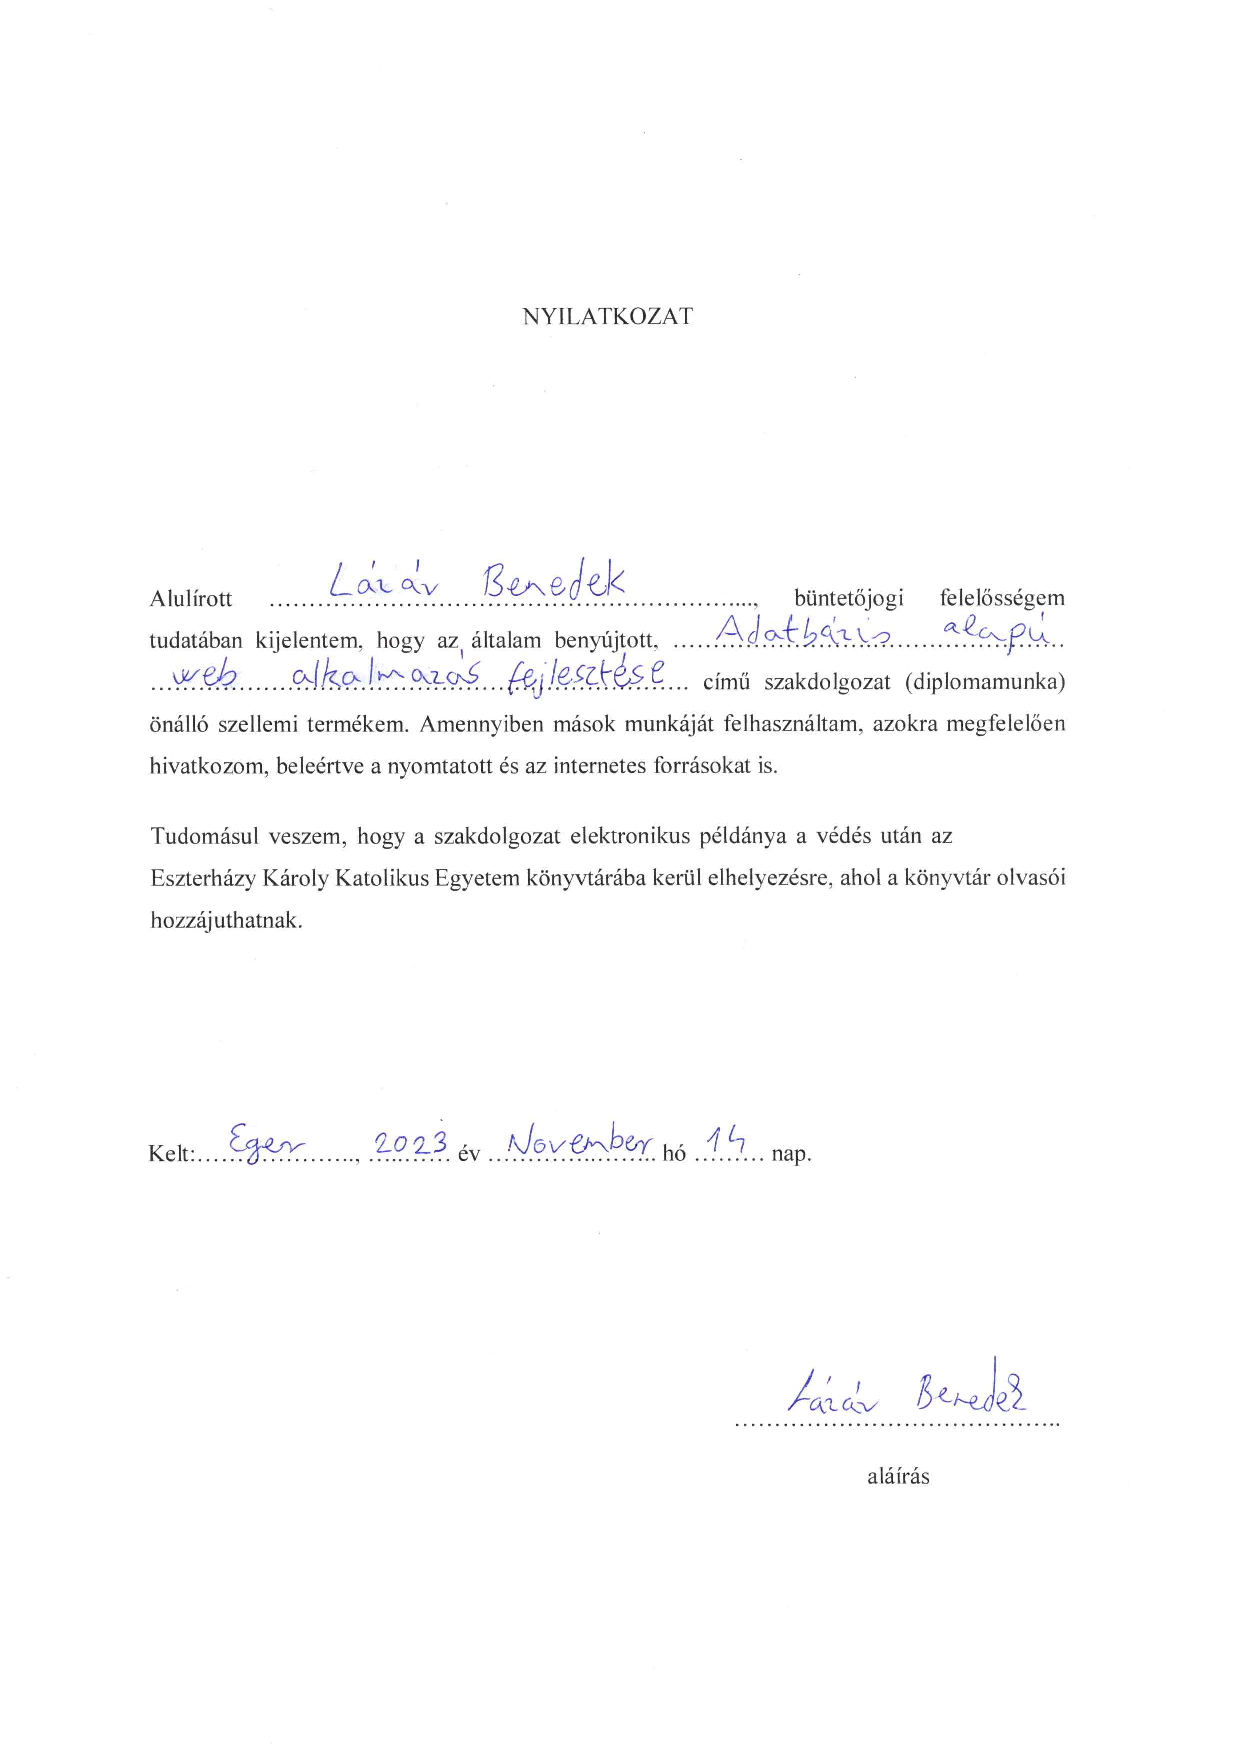
\includepdf{nyilatkozat.pdf}
\end{document}